% === T11 - Sistemas de Cómputo y su evolución ===
% David Alejandro Gonzalez Marquez
% fokerman@gmail.com
% https://github.com/fokerman/computingSystemsCourse

\documentclass[aspectratio=169]{beamer}
\usepackage{../packages}

\title{\Huge Sistemas de Cómputo y su evolución}
\author{David Alejandro González Márquez}
\institute{}

\date{}

\begin{document}

\begin{frame}[plain]
    \titlepage
    \begin{textblock}{100}(30,80)
    \begin{tcolorbox}[size=small,width=\textwidth,colback={gray!30},title={}]
    \begin{center}
     \scriptsize Clase disponible en: \url{https://github.com/fokerman/computingSystemsCourse}
    \end{center}
    \end{tcolorbox}
    \end{textblock}
%     \begin{textblock}{140}(10,70)
%     \textcolor{rojo}{
%     \textbf{Atención}: La clase será grabada por el anfitrión para su posterior y eventual uso académico dentro de nuestra institución. Su participación en la clase implica brindar su consentimiento para participar en la grabación, aunque pueden mantener su video apagado.}
%     \end{textblock}
\end{frame}

% Historia del hardware. Evolución. Primeros sistemas de cómputo. Evolución tecnológica. Máquinas mecánicas, valvulares. El transistor. Circuito integrado. Procesador. Ejemplo 4004. IBM360.

\begin{frame}[fragile,t]{Historia del hardware}
    La \textbf{evolución} de los sistemas de cómputo está guiada por \textbf{avance tecnológico}.\\
    \bigskip
    A medida que pudimos construir \textbf{sistemas más complejos},\\ fue posible materializar ideas en forma de hardware de cómputo.\\
    \bigskip
    \pause 
    Este recorrido revela cada uno de estos avances tecnológicos y\\ qué máquinas nuevas \textbf{fue posible construir}.\\
    \bigskip
    \begin{itemize}
    \item {Generación Cero} - \textcolor{verdeuca}{Mecánicas/Electromecánicas}
    \item {Primera Generación} - \textcolor{verdeuca}{Valvulares}
    \item {Segunda Generación} - \textcolor{verdeuca}{Transistores}
    \item {Tercera Generación} - \textcolor{verdeuca}{Circuitos Integrados}
    \item {Cuarta Generación} - \textcolor{verdeuca}{Integración a gran escala}
    \end{itemize}
\end{frame}

\begin{frame}[fragile,t]{Generación Cero - Mecánicas/Electromecánicas}
    \begin{textblock}{80}(3,12)
    \begin{itemize}
    \setlength\itemsep{0.1cm}
    \scriptsize
    \item<1-> \small Calculadora de Pascal (1623-1662)\\
    \scriptsize \textcolor{gray}{Calculadora, operaciones de suma y restas.} % rodillo de cobre - pascalina
    \item<1-> \small Calculadora de Leibniz (1646-1716)\\ 
    \scriptsize \textcolor{gray}{Calculadora, operaciones de suma, resta, multiplicación y división.} % Staffelwalze
    \item<2-> \small Máquina diferencial de Babbage (1847-1849)\\
    \scriptsize \textcolor{gray}{Calculadora de propósito específico: método de diferencias finitas utilizando polinomios.}
    \item<2-> \small Máquina analítica de Babbage (1837-1871)\\
    \scriptsize \textcolor{gray}{Máquina de propósito general: leía instrucciones de tarjetas perforadas y las ejecutaba.}
    \item<3-> \small Máquina de Atanasoff (1940)\\
    \scriptsize \textcolor{gray}{Calculadora de aritmética binaria y memoria de capacitores.}
    \item<3-> \small Máquina de Zuse, Z1 (1944)\\
    \scriptsize \textcolor{gray}{Primera computadora electromecánica, basada en reles y destruida durante la segunda guerra.}
    \item<3-> \small Máquina de Aiken, Mark 1 (1944)\\
    \scriptsize \textcolor{gray}{Diseño Harvard, 1 instrucción cada 6 segundos. E/S en cinta de papel y tarjeta perforadas.}
    % -> calculadoras automaticas -> entrada secuencial de instrucciones -> limitadas posibilidades de cambiar la secuencia de operaciones
    \end{itemize}
    \end{textblock}
    \begin{textblock}{100}(97,8)
    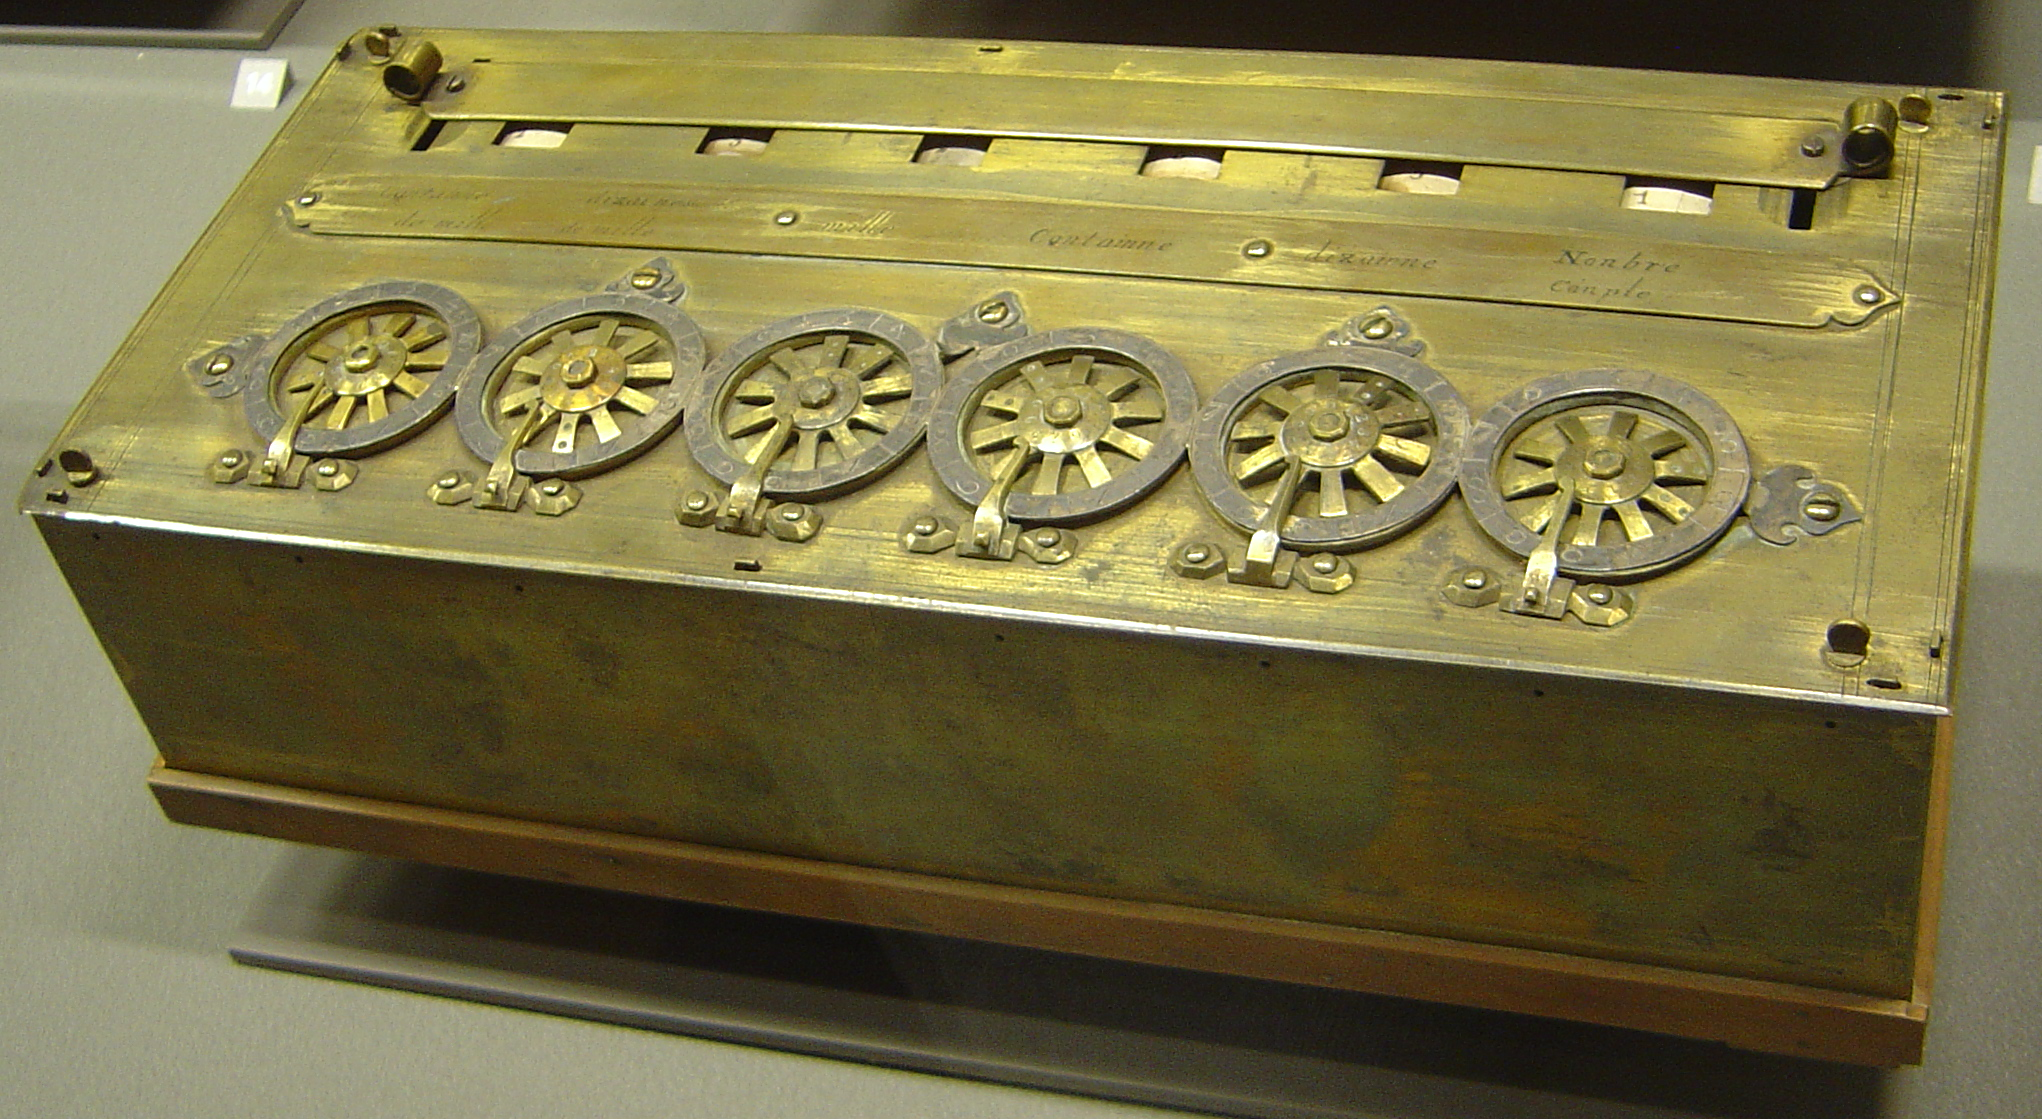
\includegraphics[height=1.8cm]{img/Pascaline.jpg} \hspace{0.1cm} 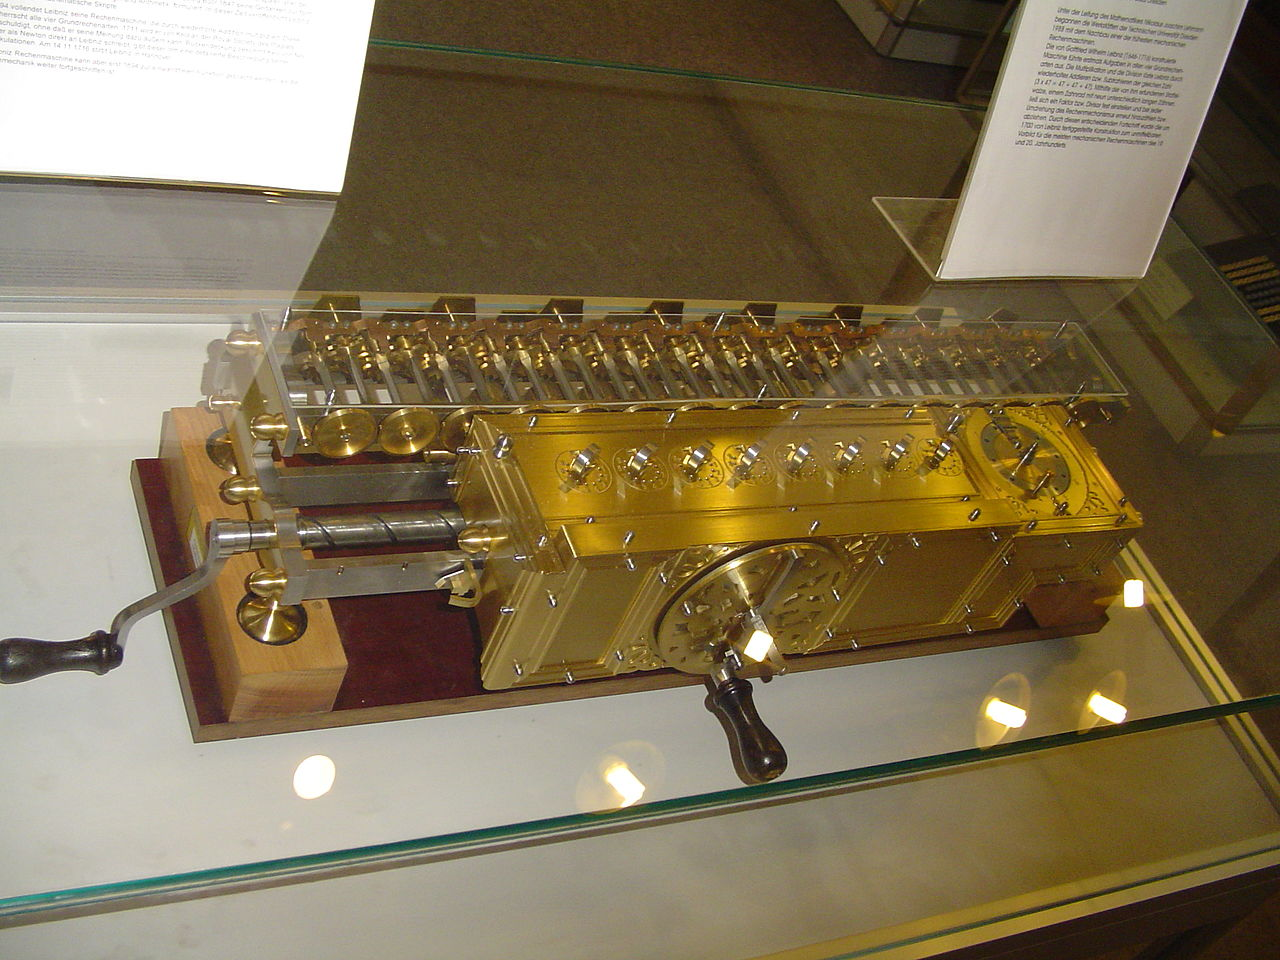
\includegraphics[height=1.8cm]{img/Leibnitzrechenmaschine.jpg}\\
    \vspace{0.1cm}
    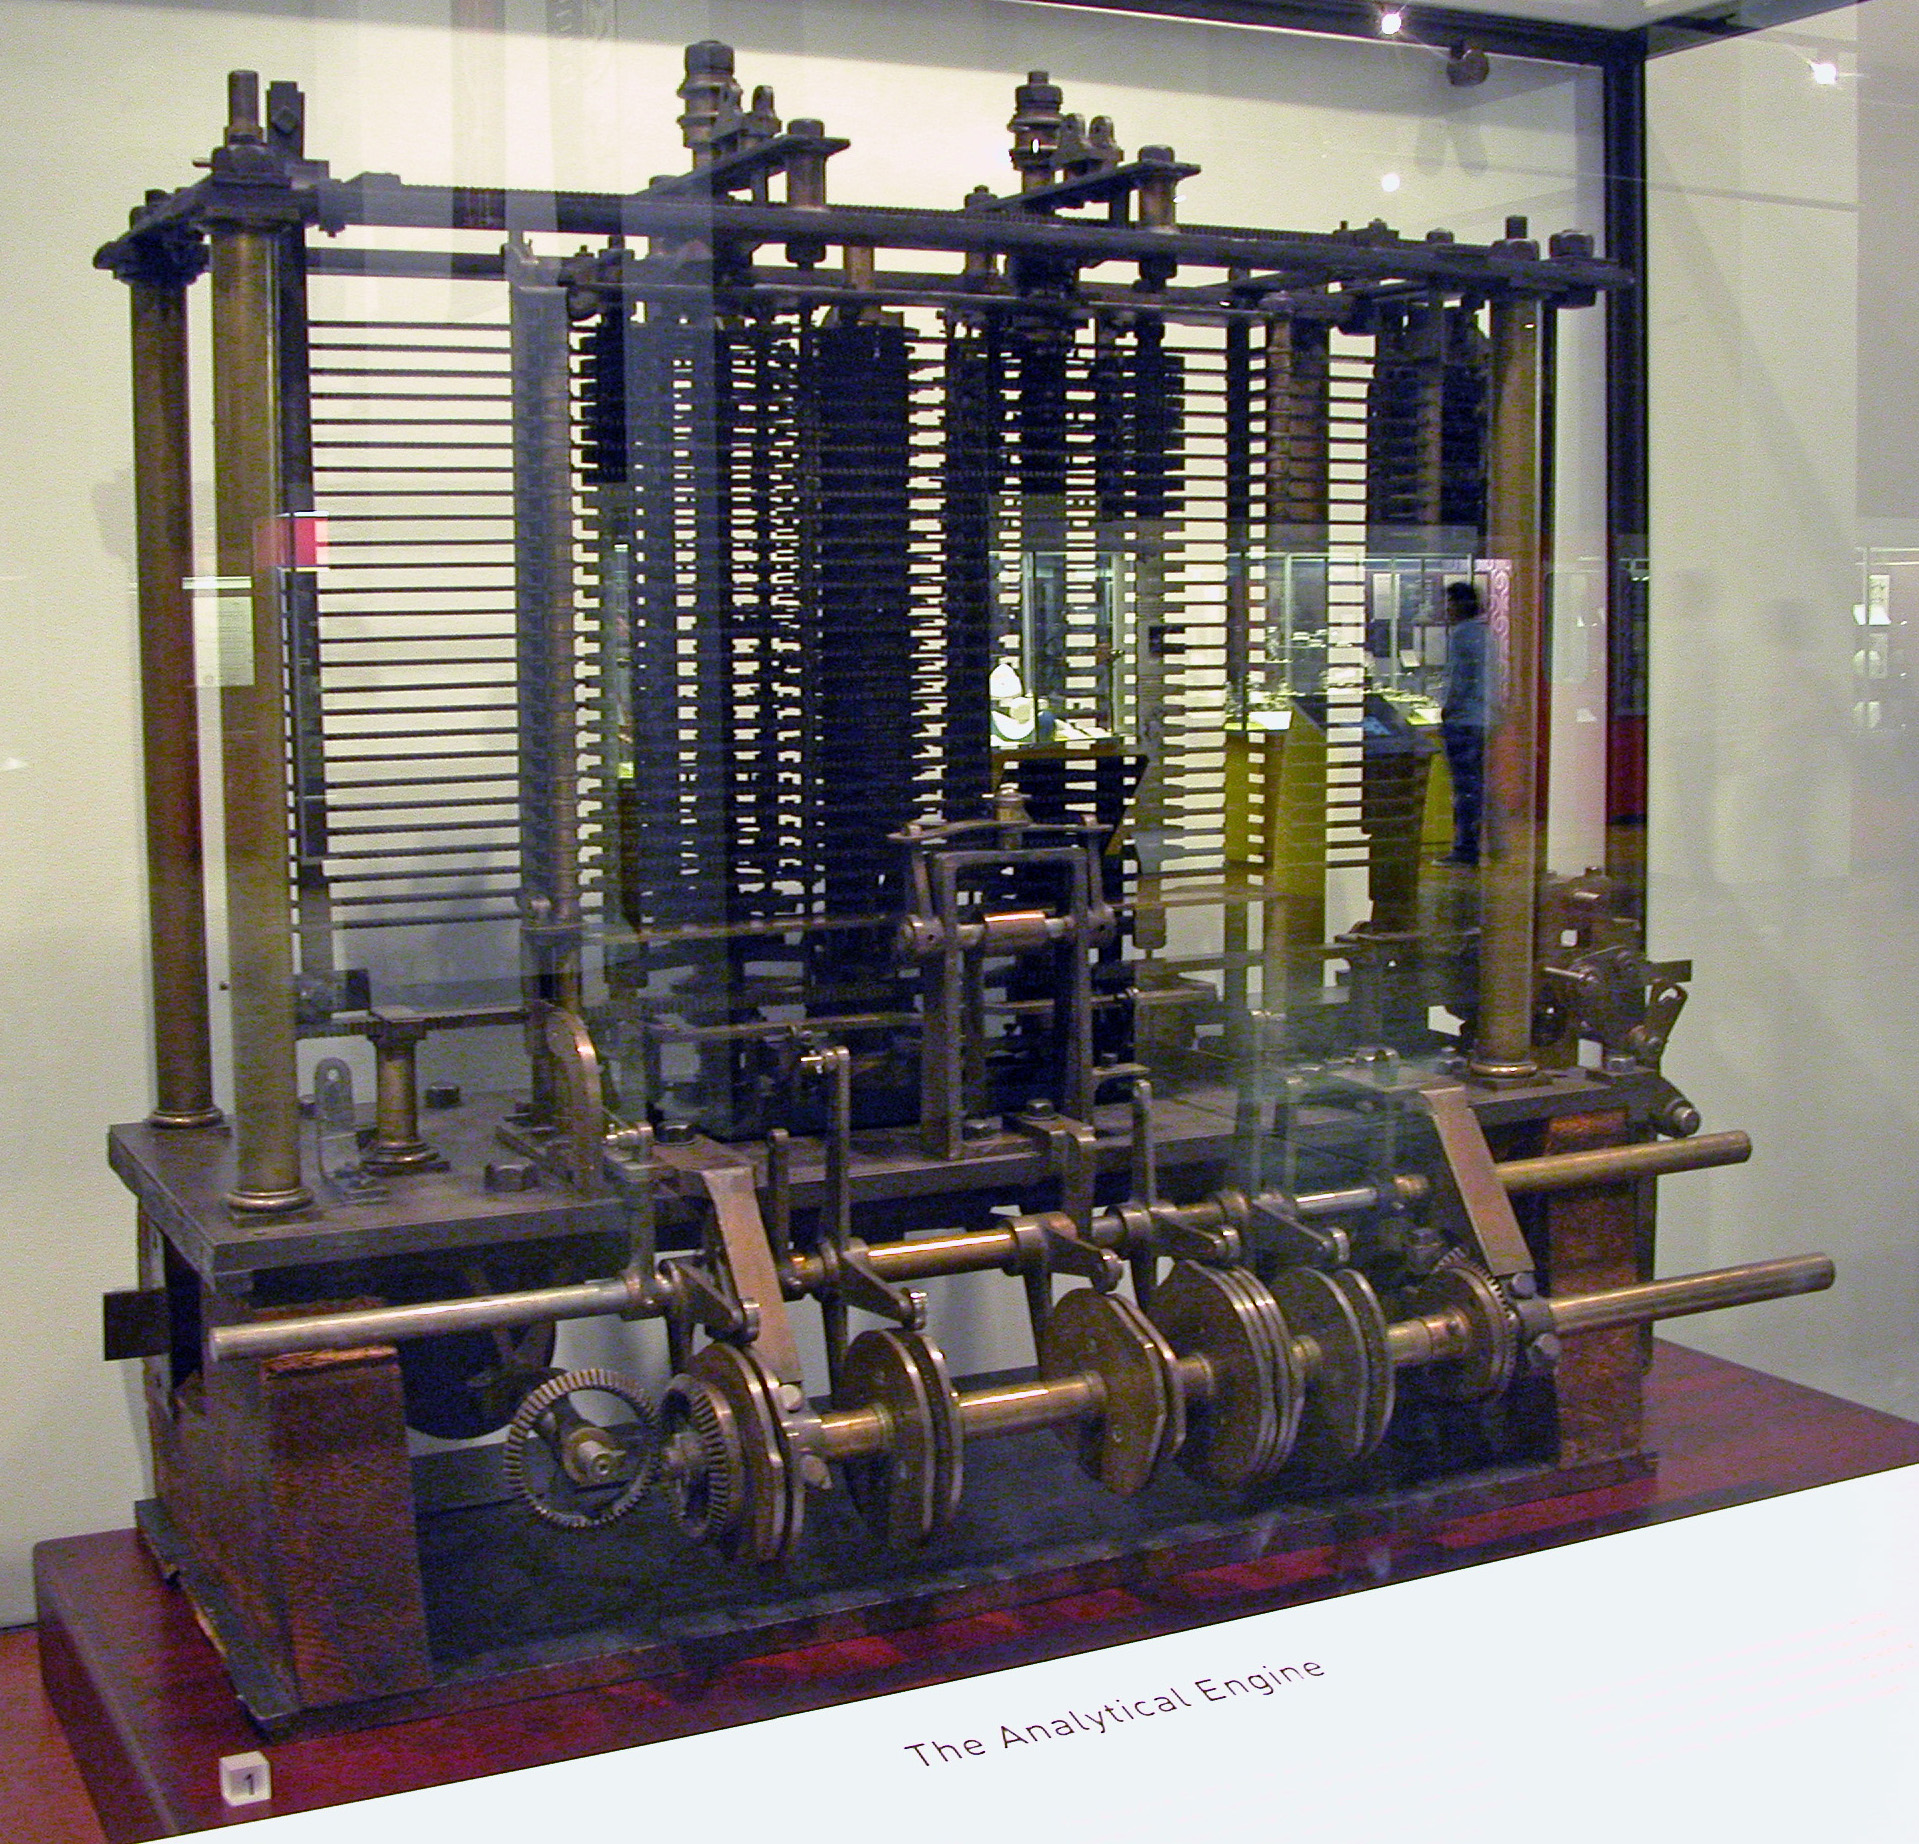
\includegraphics[height=2.44cm]{img/AnalyticalMachine_Babbage_London.jpg} \hspace{0.1cm} 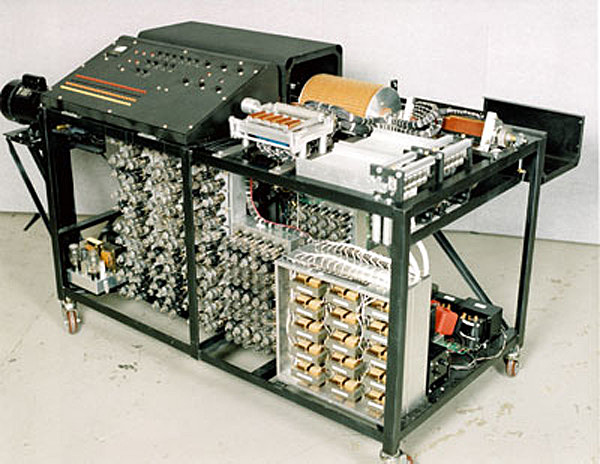
\includegraphics[height=2.44cm]{img/Atanasoff.jpg}\\
    \vspace{0.1cm}
    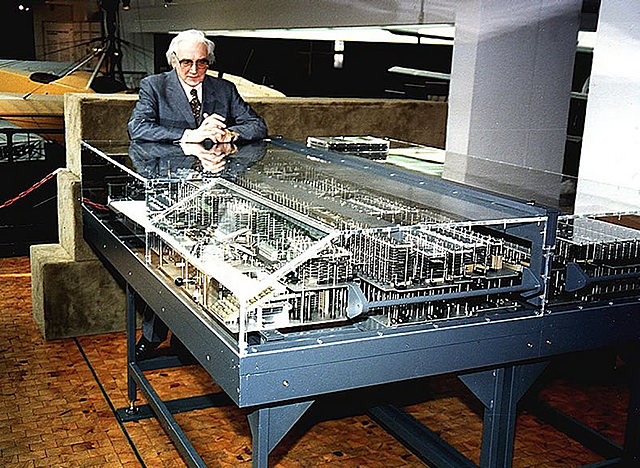
\includegraphics[height=2.9cm]{img/zuse.jpg} \hspace{0.1cm} 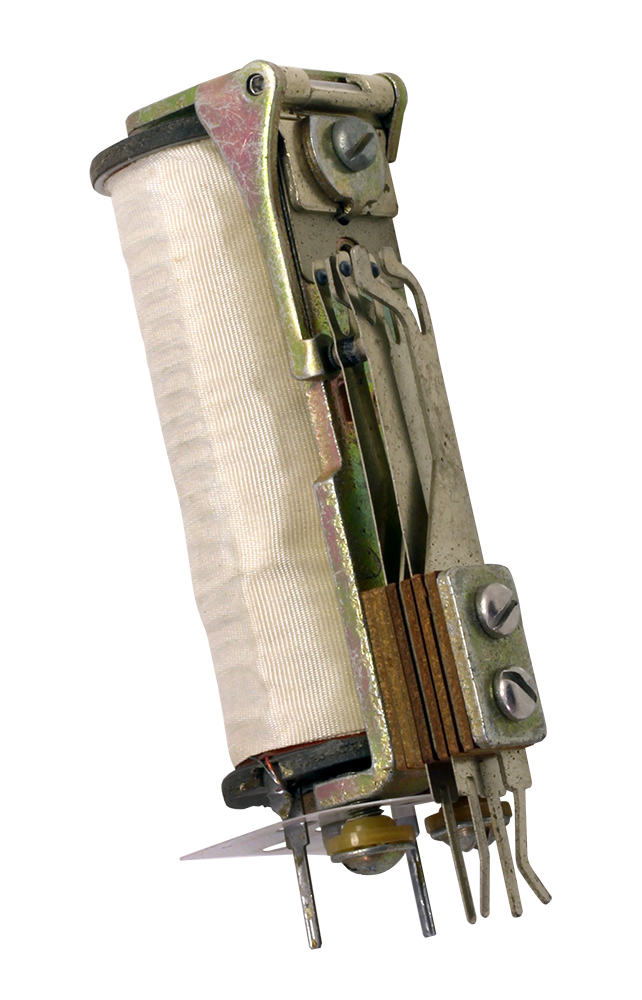
\includegraphics[height=2.9cm]{img/rele.jpg}\\
    \end{textblock}
\end{frame}

\begin{frame}[fragile,t]{Primera Generación - Valvulares}
% ***** Valvulas -> Anodo, catodo, filamento regilla ?
    \begin{textblock}{80}(3,12)
    \begin{itemize}
    \setlength\itemsep{0.2cm}
    \item<1-> Colossus (1944)\\
    \textcolor{gray}{Sistema de cómputo para romper el código Enigma (Alan Turing).}
    \item<2-> ENIAC (1946)\\ {\scriptsize Electronic Numerical Integrator And Computer}\\
    \textcolor{gray}{Cálculo de tablas balísticas, programa almacenado en interruptores, 20 registros decimales.}
    \item<3-> IAS (1951)\\
    \textcolor{gray}{Usaba binario y programa almacenado\\ (John von Neumann).}
    \item<4-> IBM 701 (1953) 704 (1956) 709 (1958)\\
    \textcolor{gray}{Contaba con una memoria de núcleos.}
    \end{itemize}
    \end{textblock}
    \begin{textblock}{100}(80,8)
    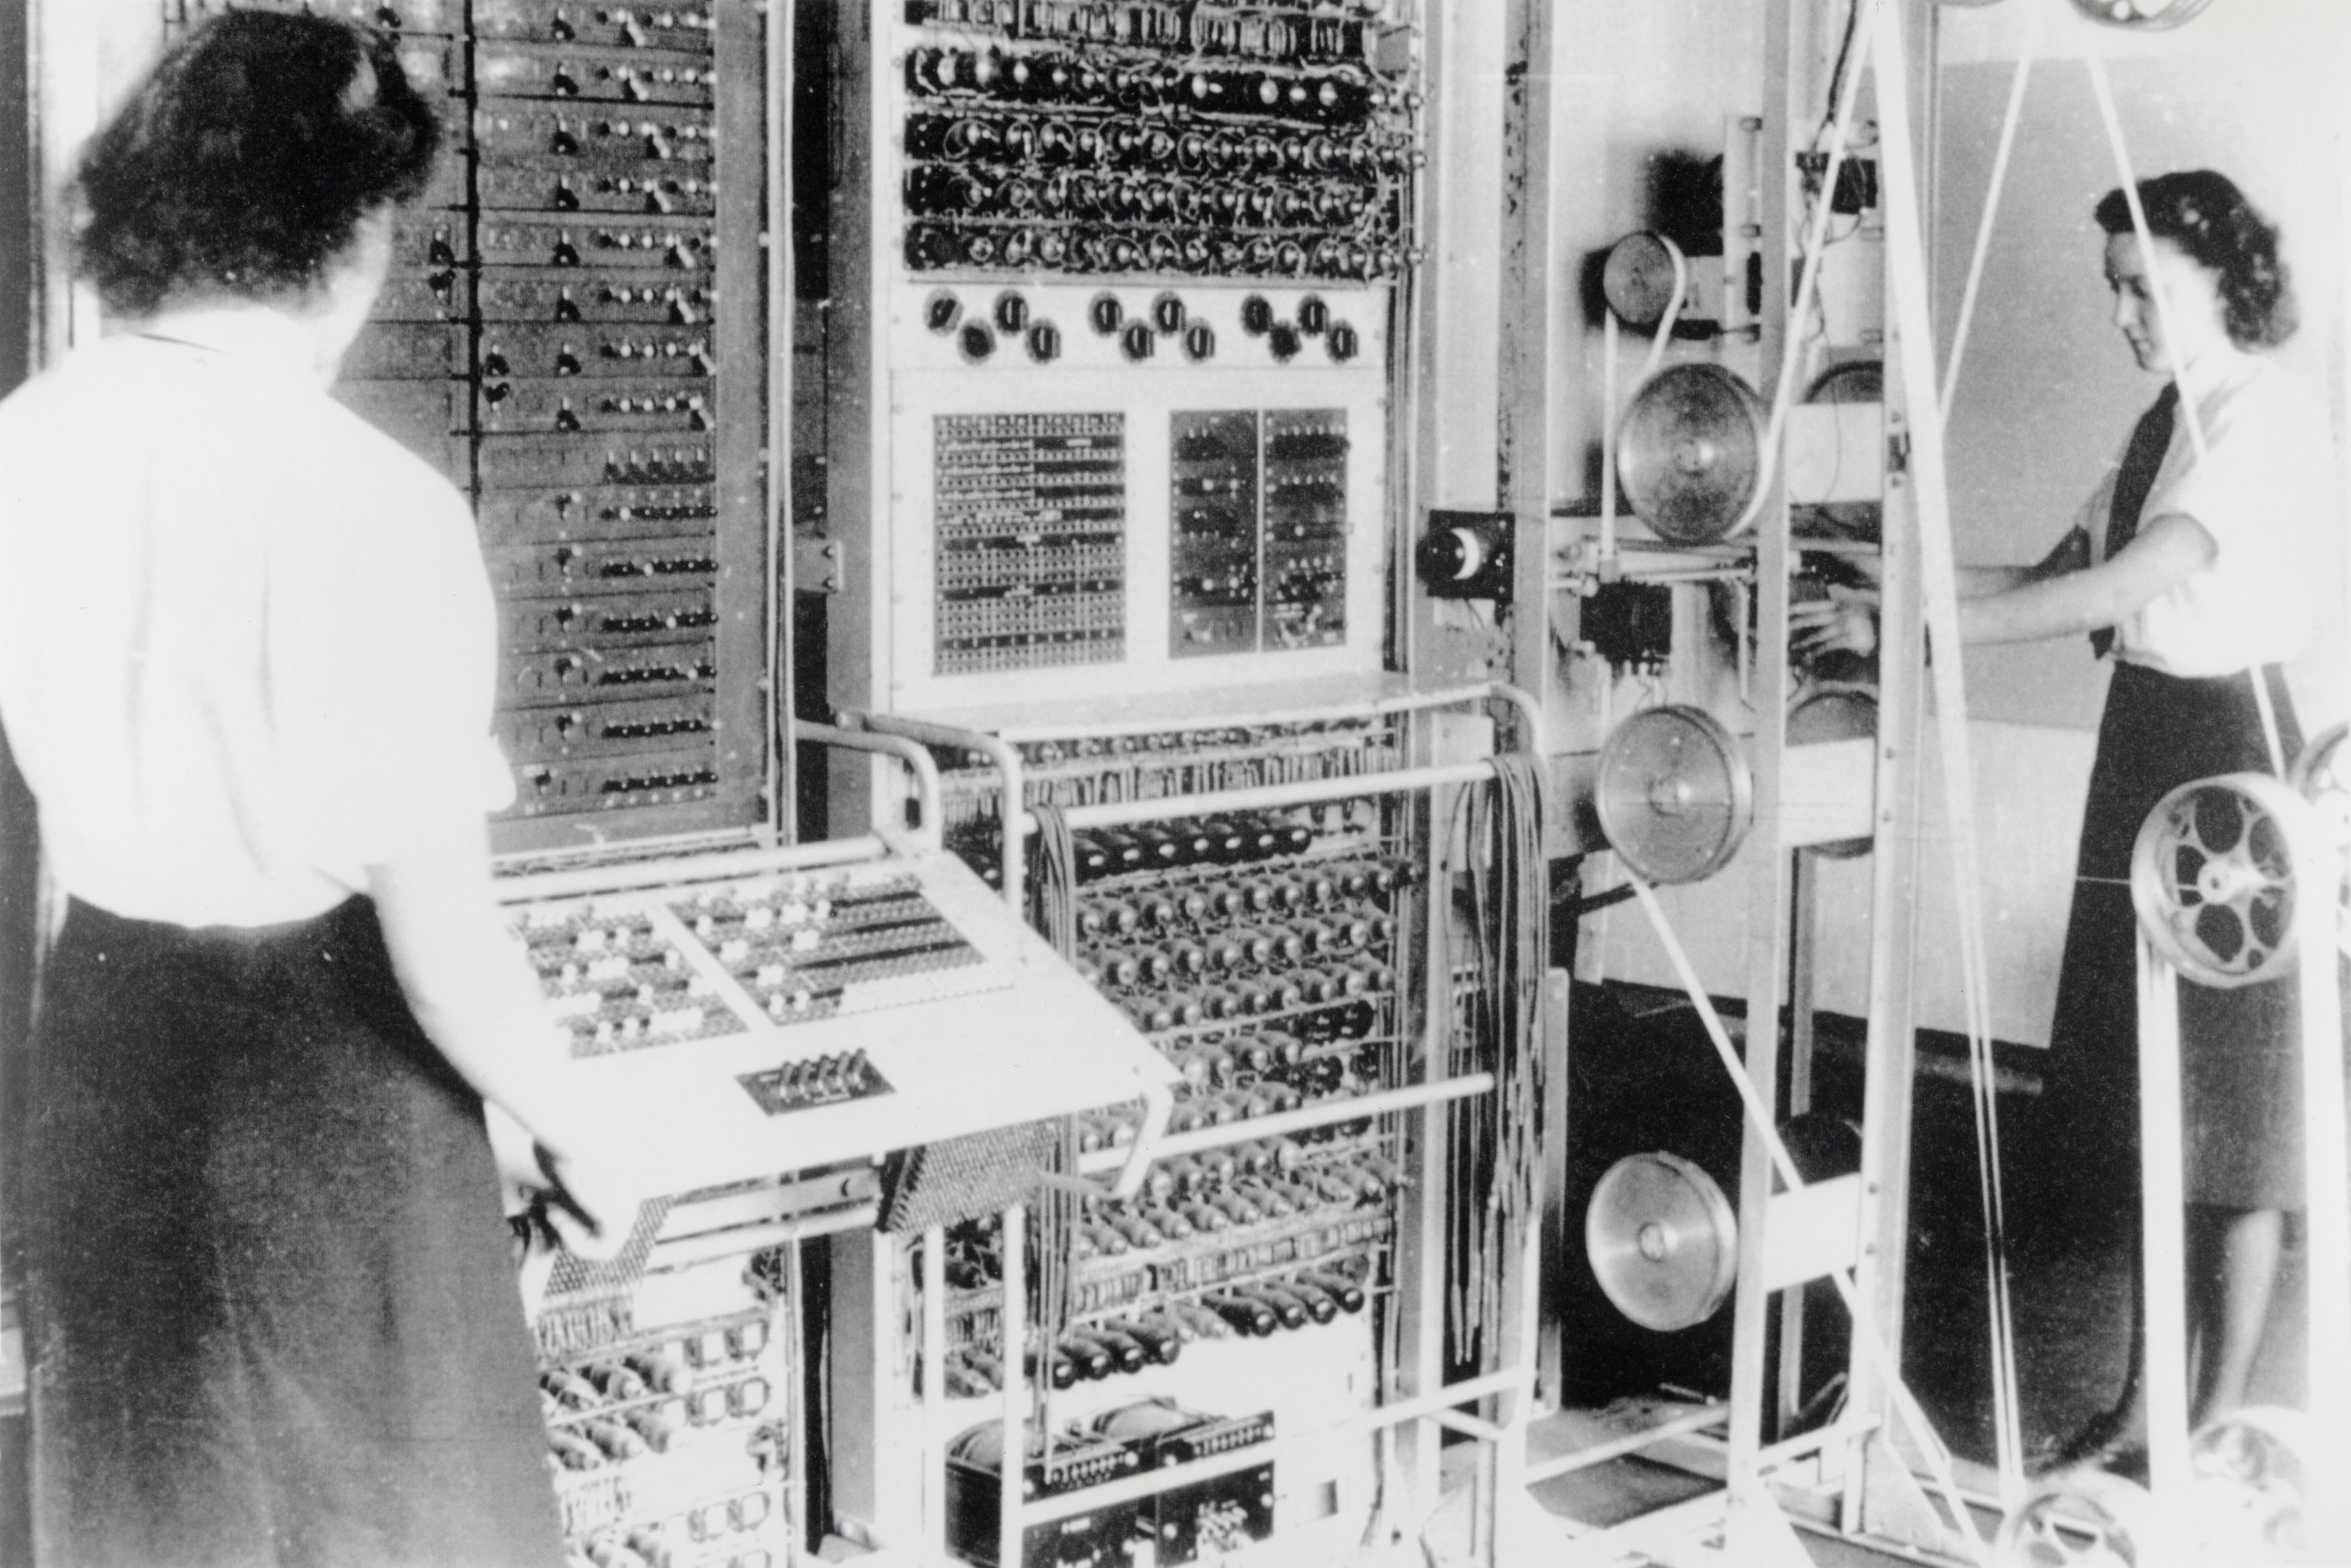
\includegraphics[height=2.23cm]{img/Colossus.jpg} \hspace{0.1cm} 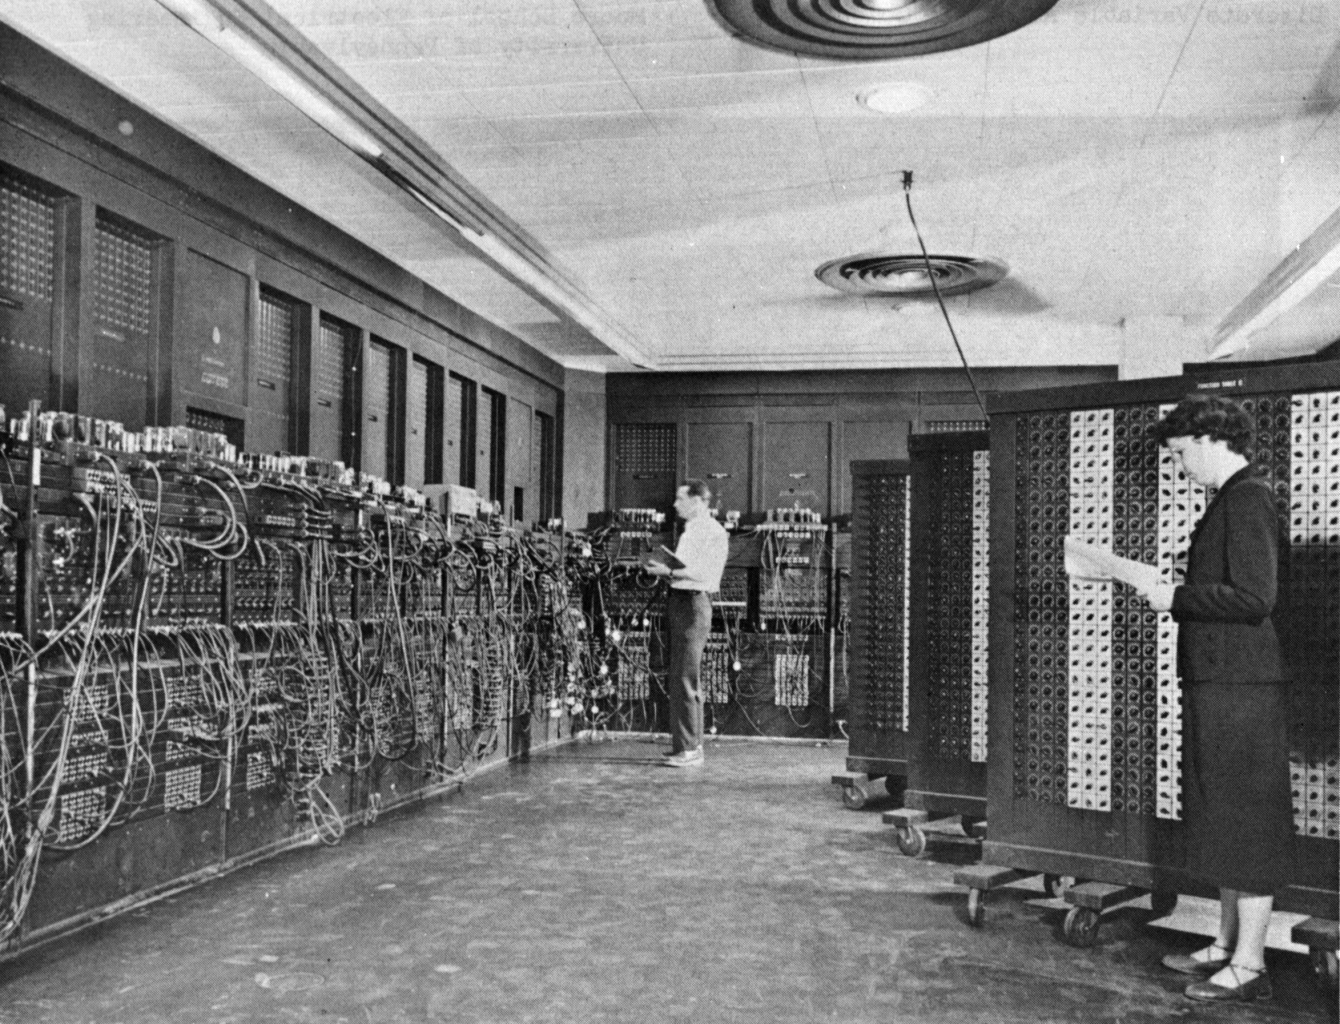
\includegraphics[height=2.23cm]{img/Eniac.jpg}
    \hspace{0.1cm} 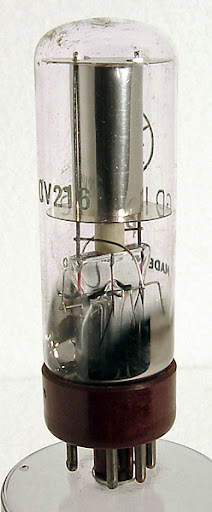
\includegraphics[height=2.23cm]{img/valve.jpg}\\
    \vspace{0.1cm}
    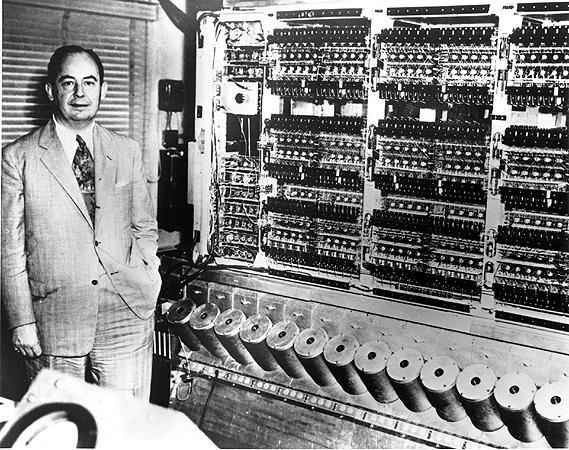
\includegraphics[height=2.44cm]{img/ias.jpg} \hspace{0.1cm} 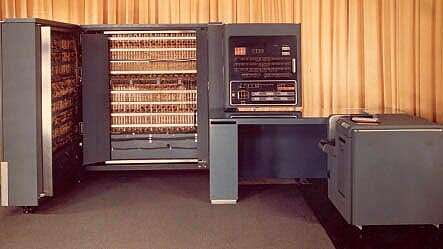
\includegraphics[height=2.44cm]{img/IBM701.jpg}\\
    \vspace{0.1cm}
    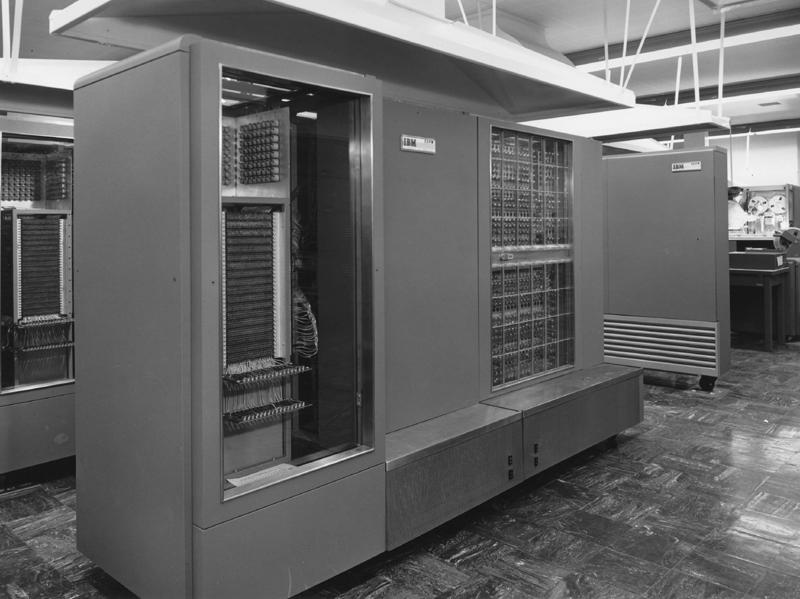
\includegraphics[height=2.86cm]{img/IBM704a.jpg} \hspace{0.1cm} 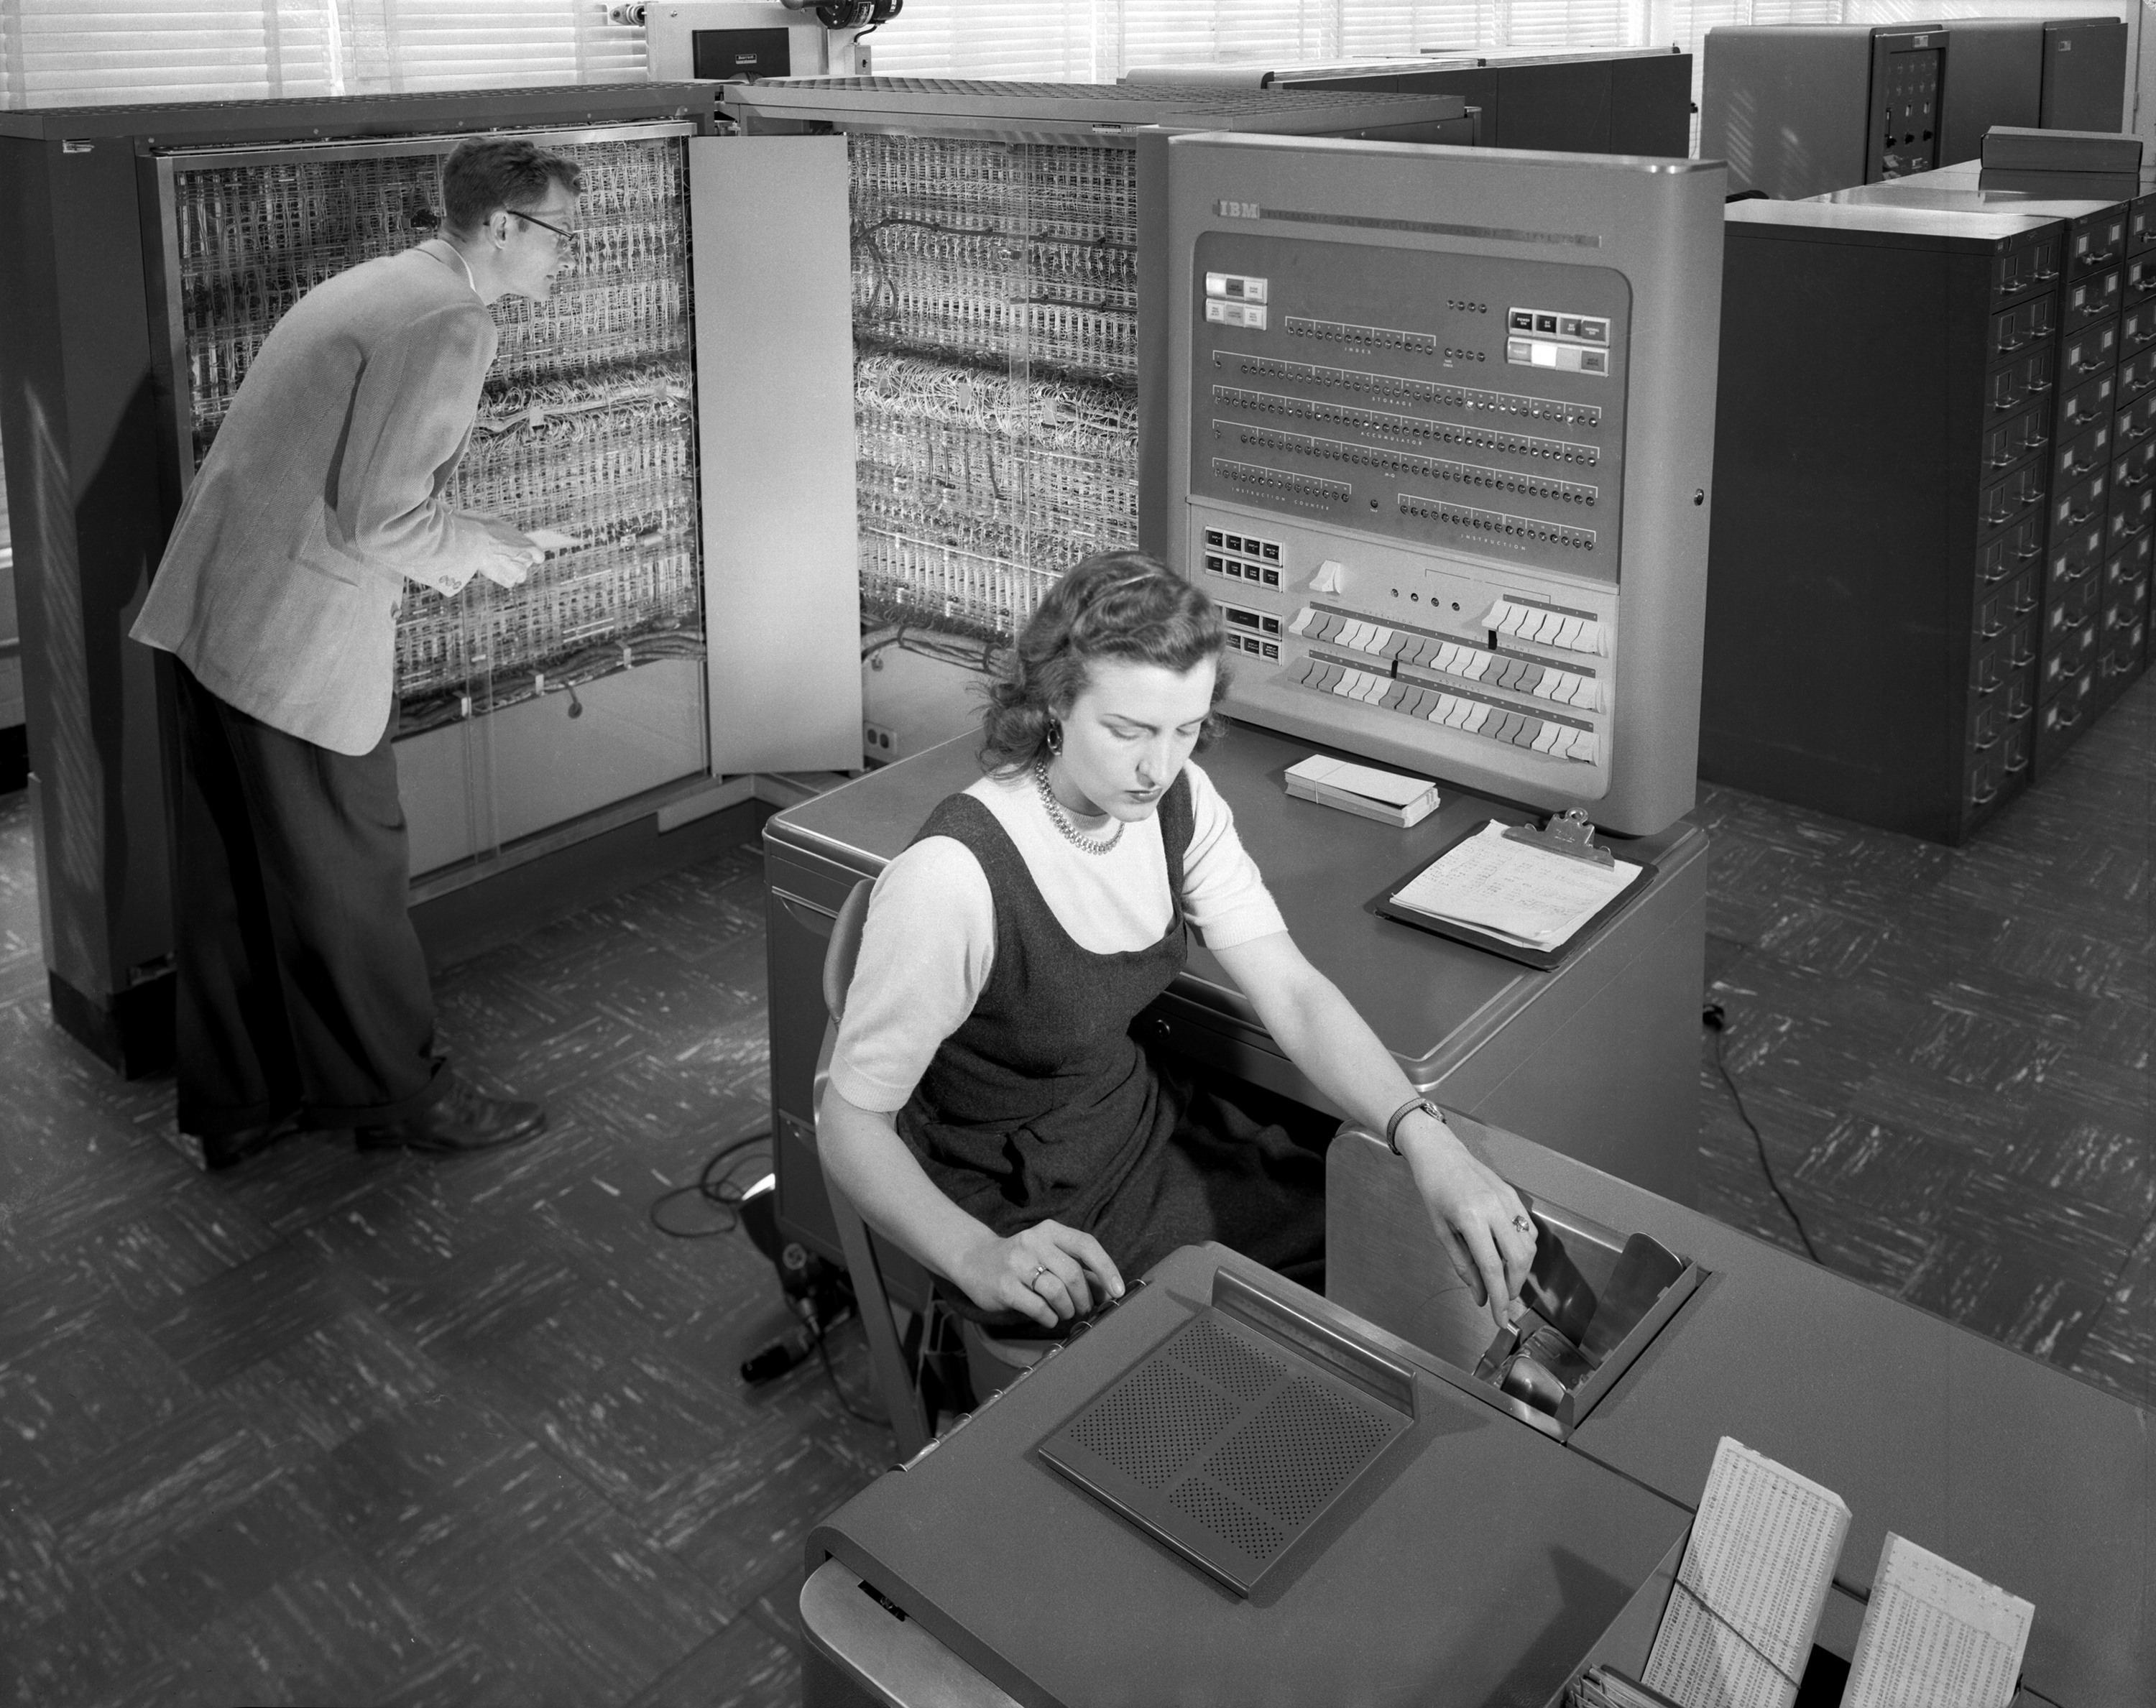
\includegraphics[height=2.86cm]{img/IBM704.jpg}\\
    \end{textblock}
\end{frame}

\begin{frame}[fragile,t]{Segunda Generación - Transistores}
% ***** Transistor -> Bell Labs 1948 -> base colector emisor
    \begin{textblock}{80}(3,12)
    \begin{itemize}
    \setlength\itemsep{0.2cm}
    \item<1-> MIT TX-0 (1956)\\
    \textcolor{gray}{Computadora transistorizada experimental.}
    \item<1-> IBM 7090 (1959)\\ 
    \textcolor{gray}{Versión transistorizada de la 709.}
    \item<2-> DEC PDP-1 (1960) {\small (Digital Equipament Corporation)}
    \textcolor{gray}{Costo de 120 mil dólares, 4k palabras de 18bits, memoria de núcleos.}
    \item<2-> DEC PDP-8 (1965)\\
    \textcolor{gray}{Costo de 16 mil dólares, palabra de 12 bits, bus único de conexión.}
    \item<2-> CDC 6600 (1965) {\small (Control Data Corporation)}\\
    \textcolor{gray}{Múltiples unidades funcionales, procesadores auxiliares, Arquitectura RISC (Seymour Cray).}
    \end{itemize}
    \end{textblock}
    \begin{textblock}{100}(85,8)
    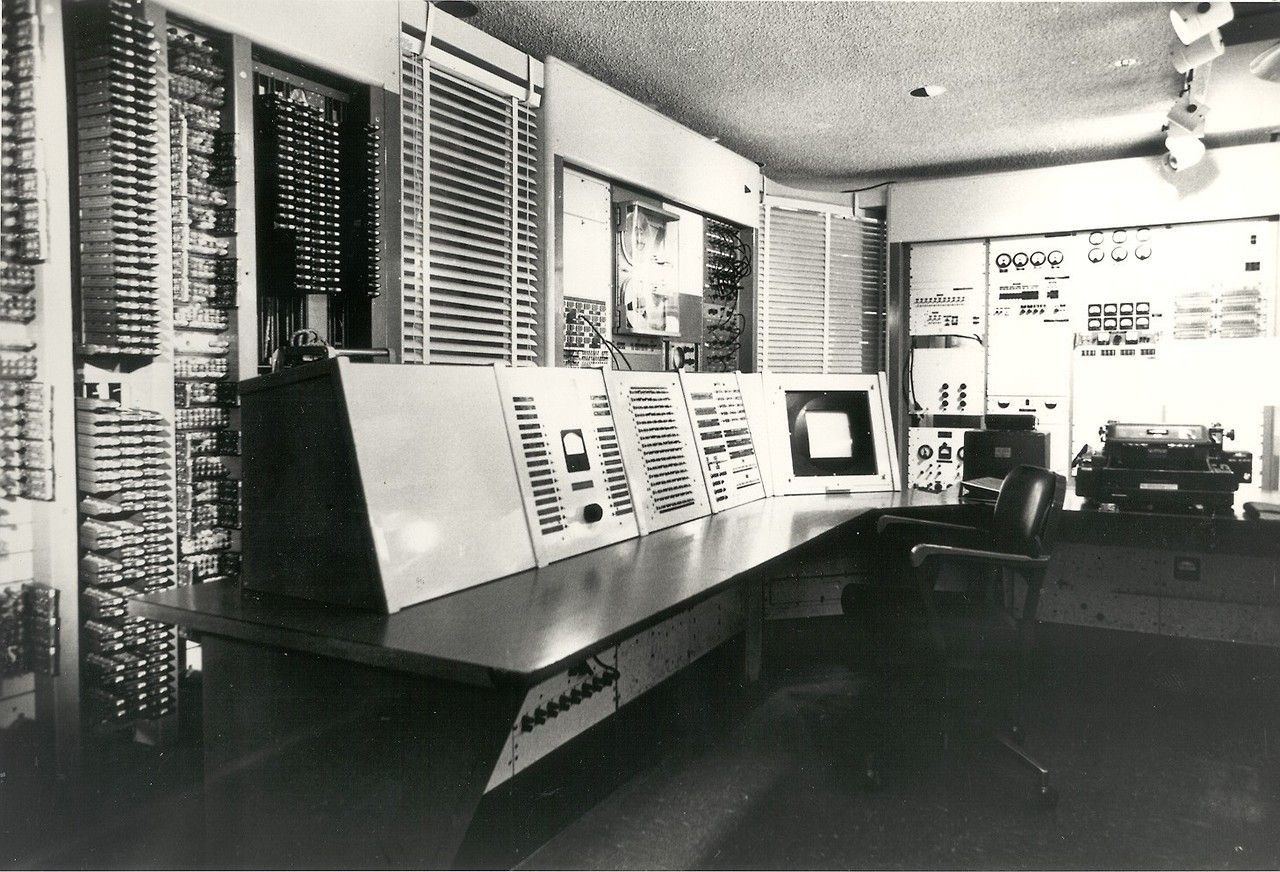
\includegraphics[height=2.26cm]{img/MIT-TX-0.jpg} \hspace{0.1cm} 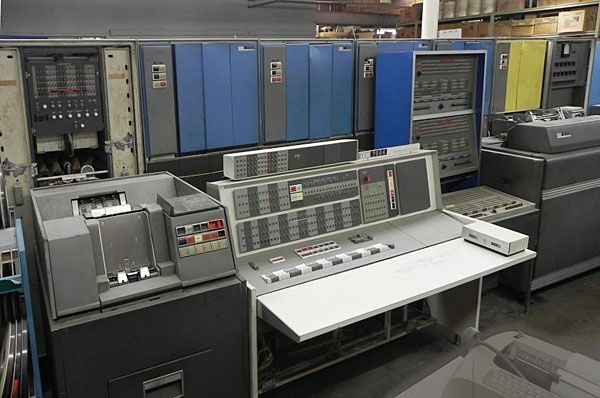
\includegraphics[height=2.26cm]{img/IBM7094.jpg}\\
    \vspace{0.1cm}
    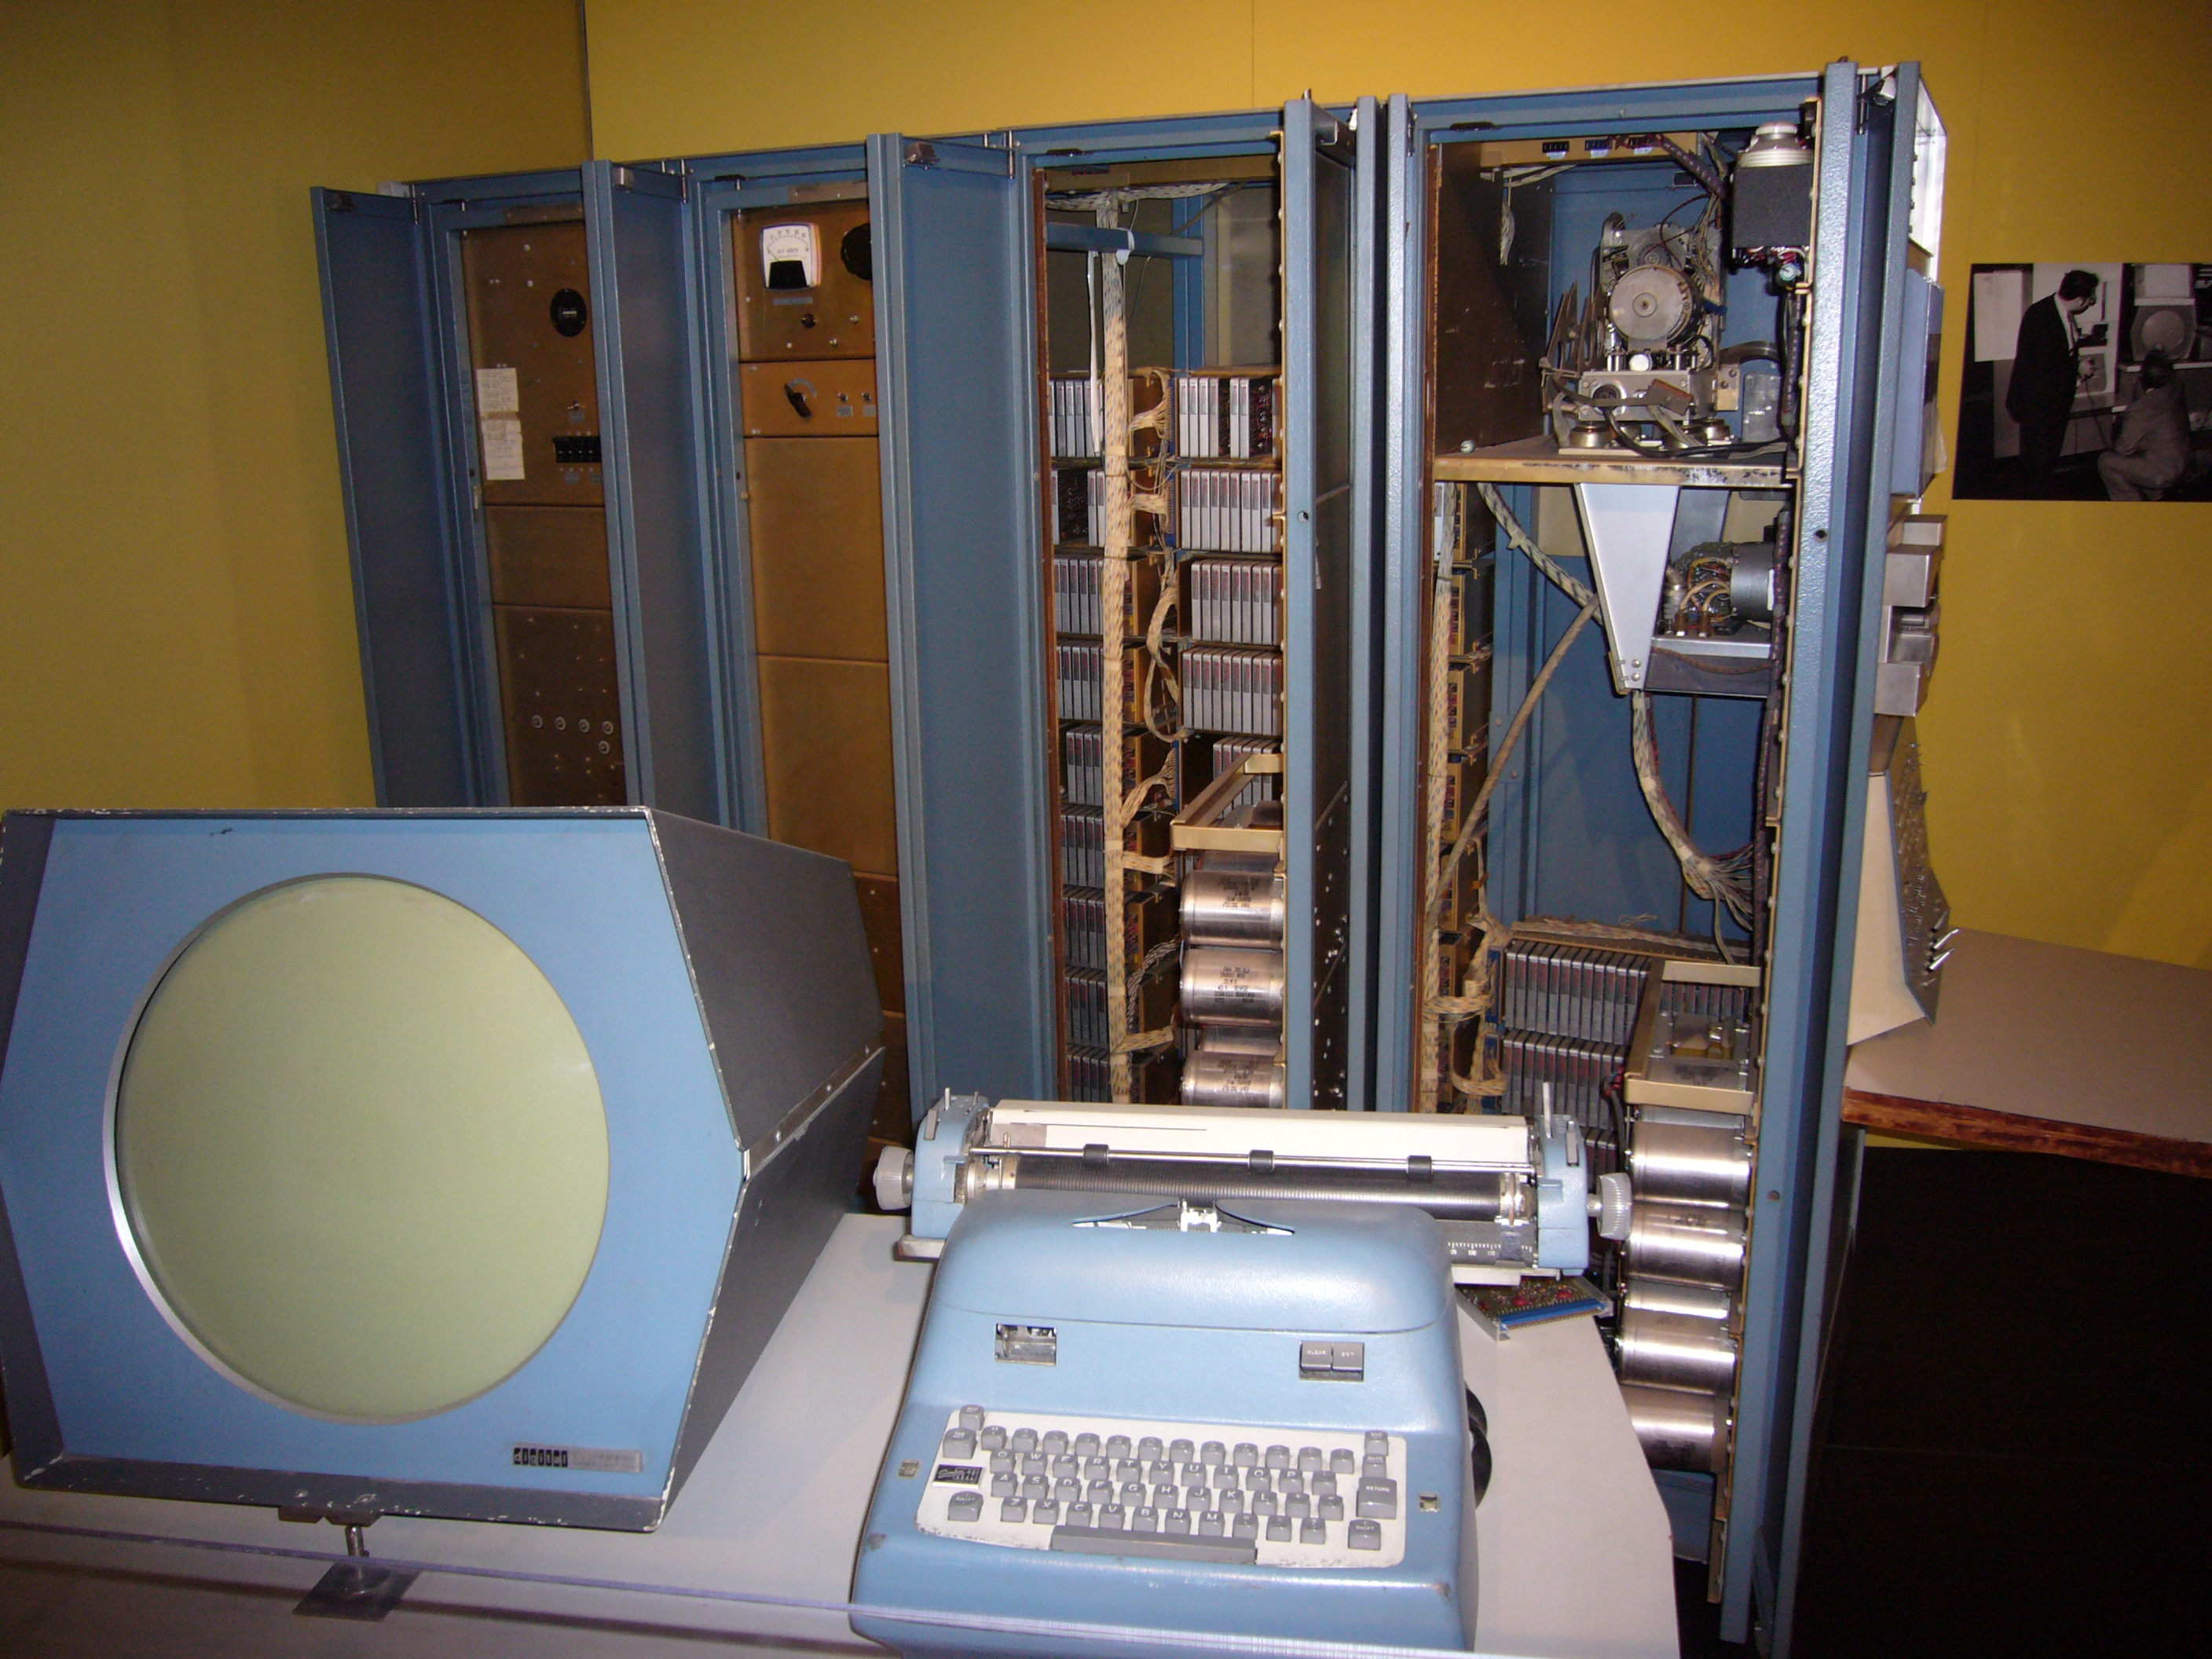
\includegraphics[height=2.3cm]{img/PDP-1.jpg} \hspace{0.1cm} 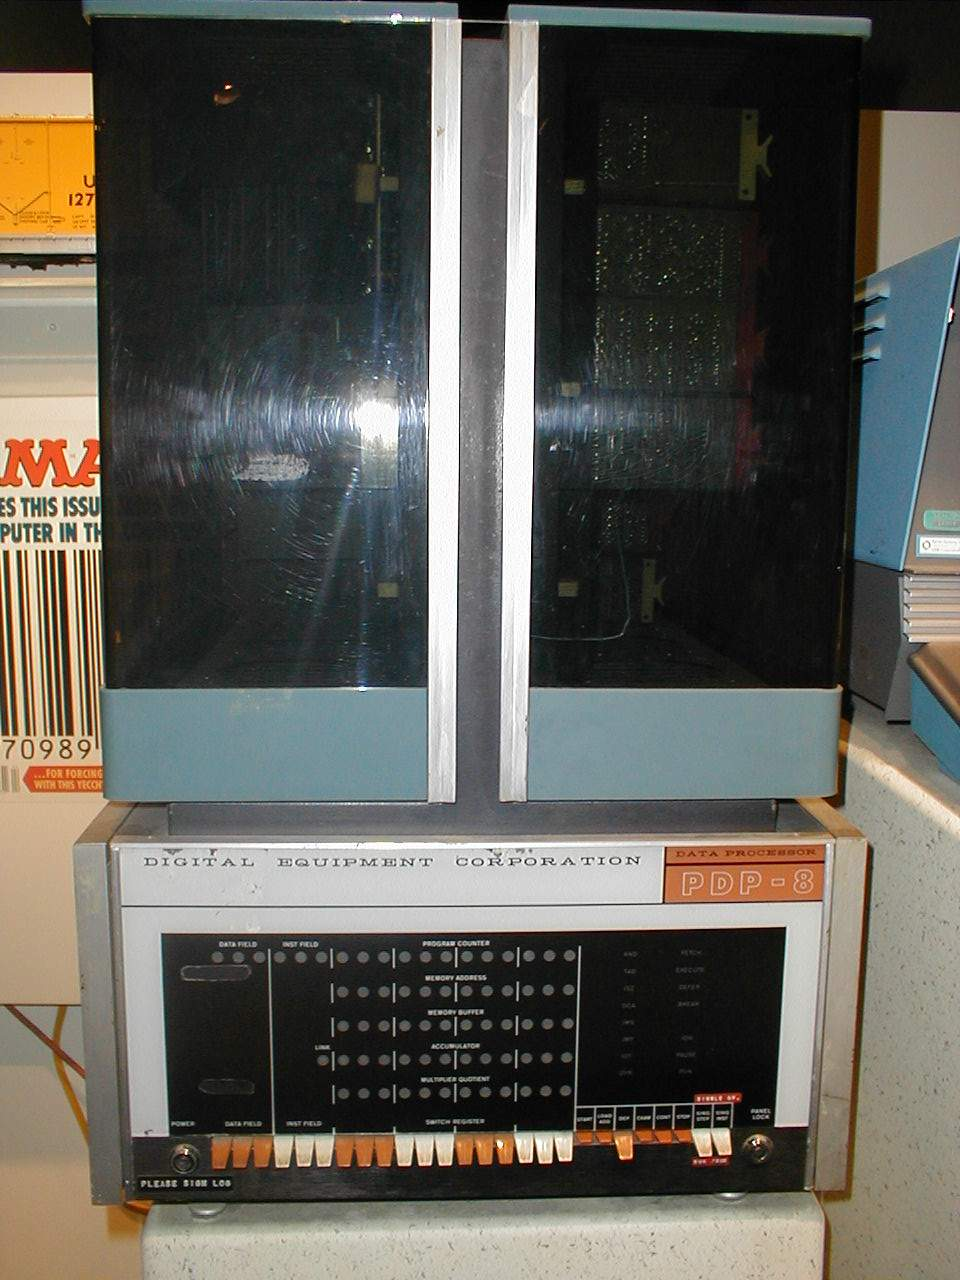
\includegraphics[height=2.3cm]{img/PDP-8.jpg}  \hspace{0.1cm} 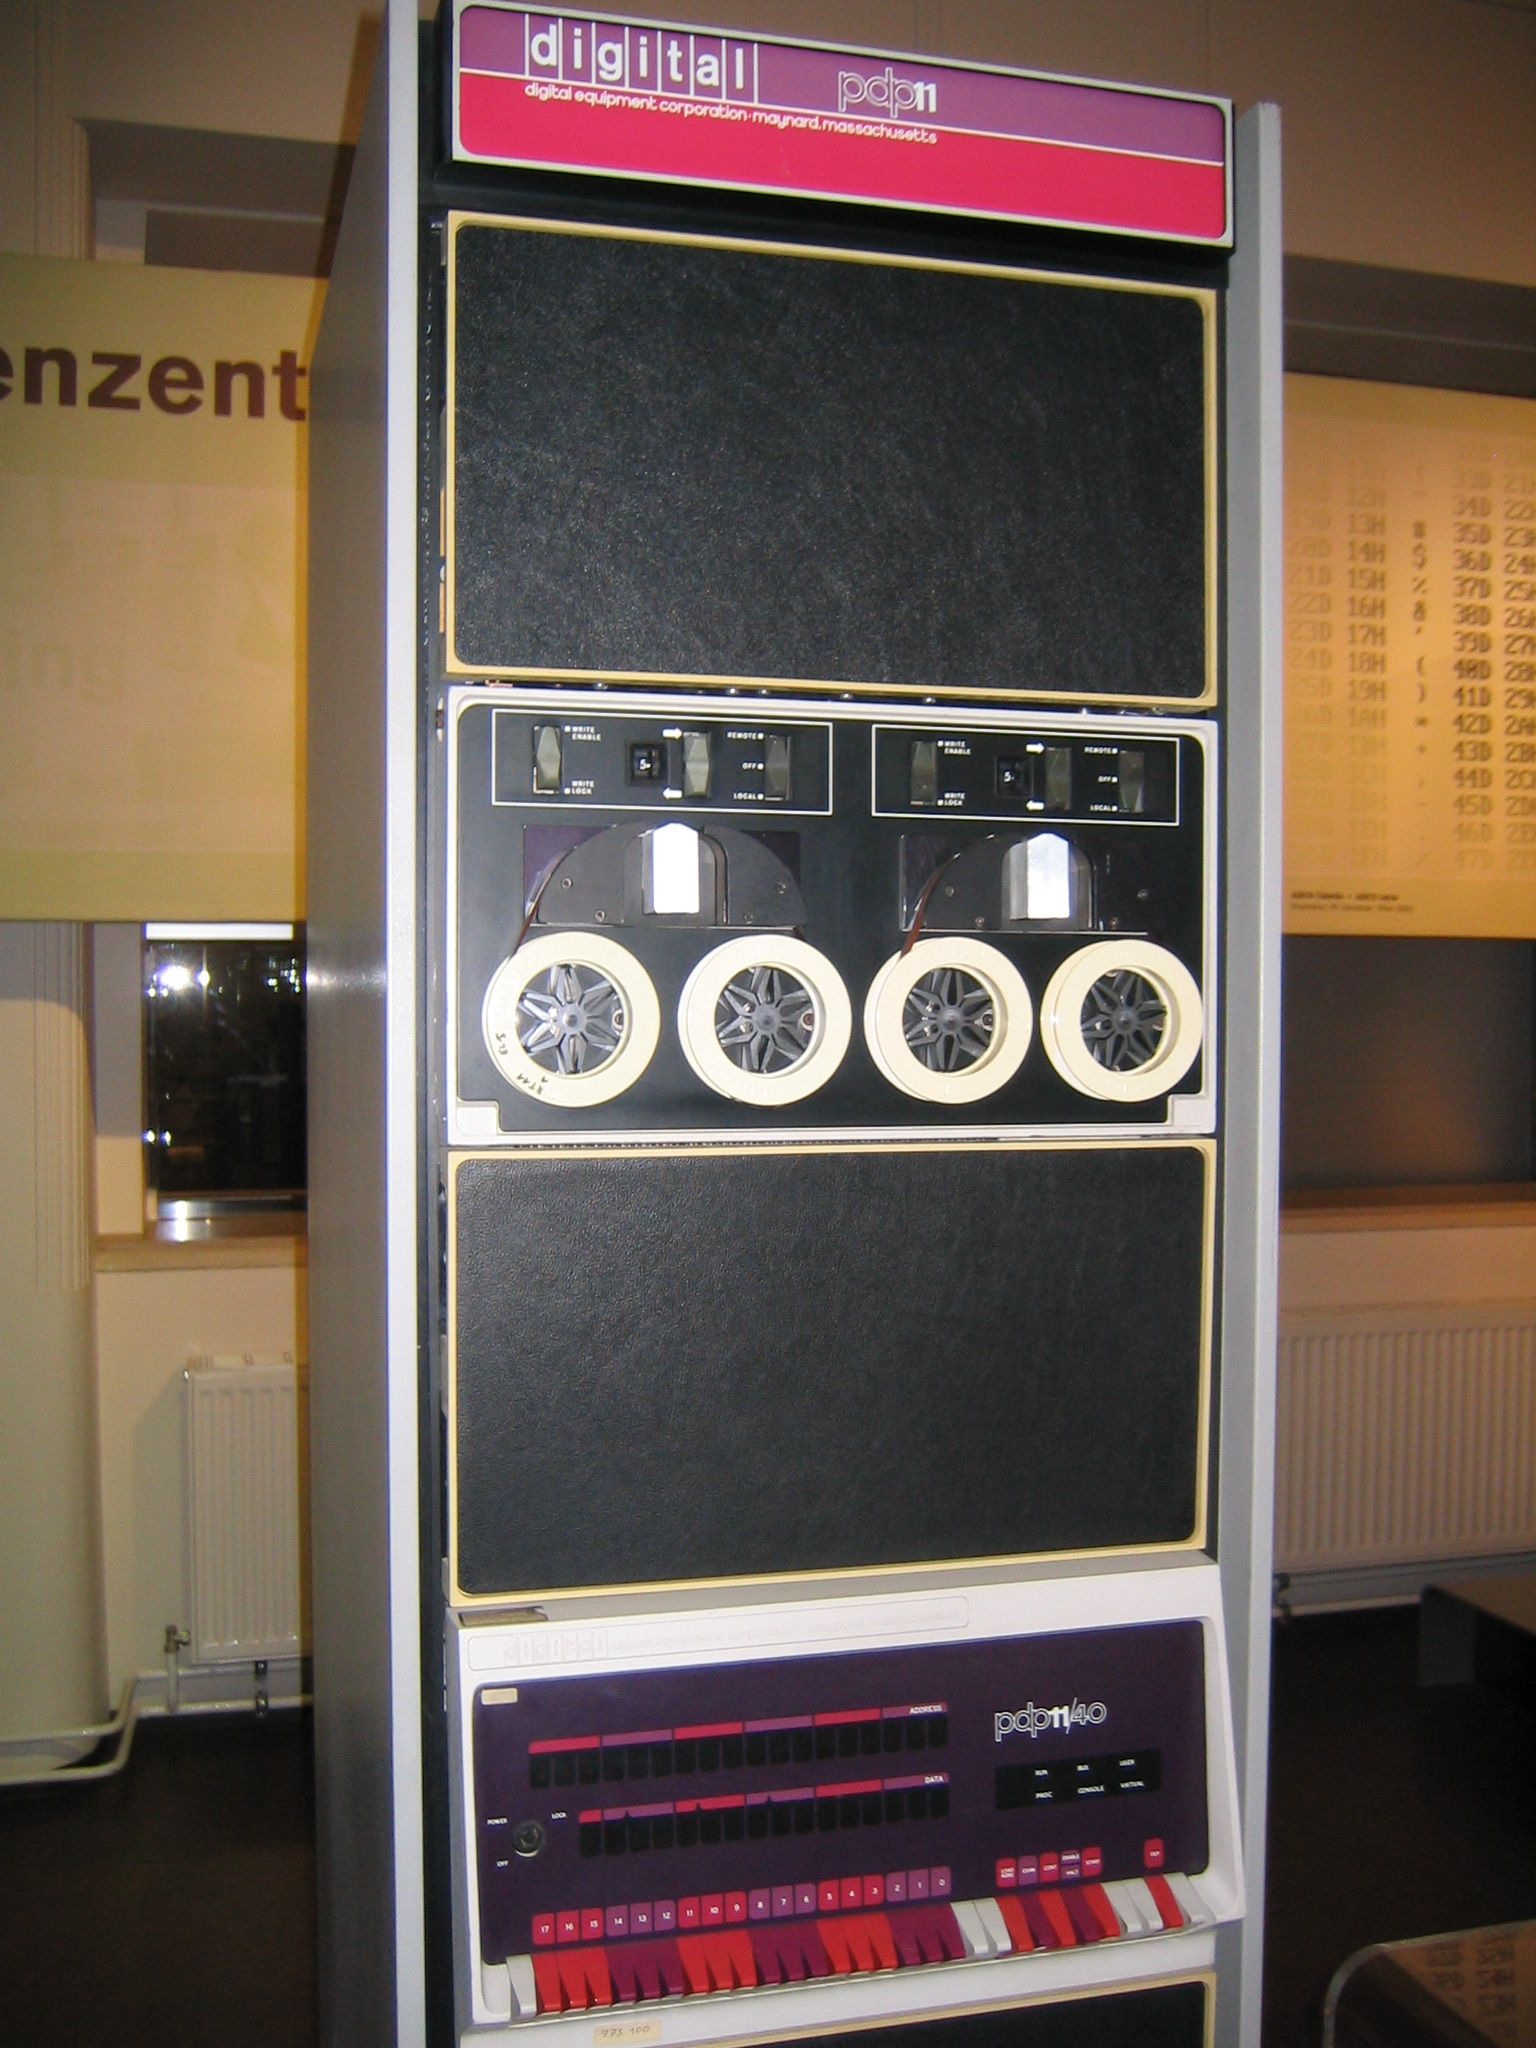
\includegraphics[height=2.3cm]{img/PDP-11.jpg}\\
    \vspace{0.1cm}
    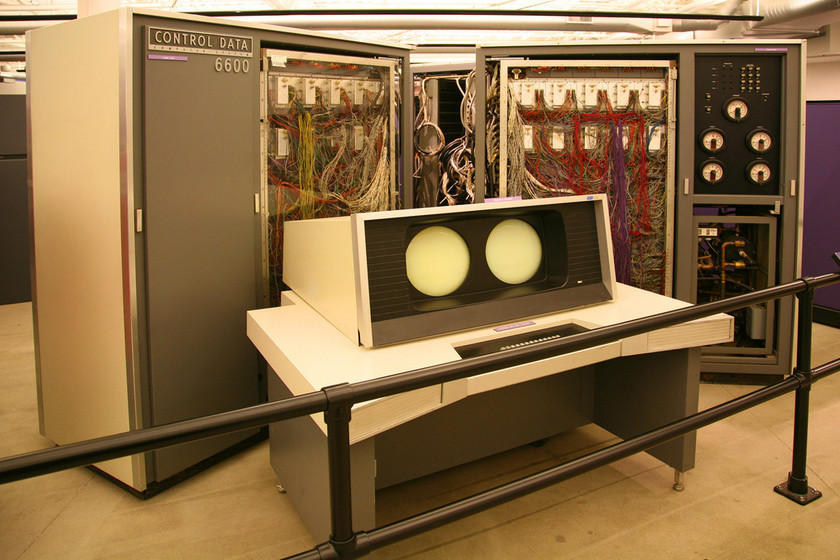
\includegraphics[height=2.63cm]{img/CDC6600.jpg} \hspace{0.1cm} 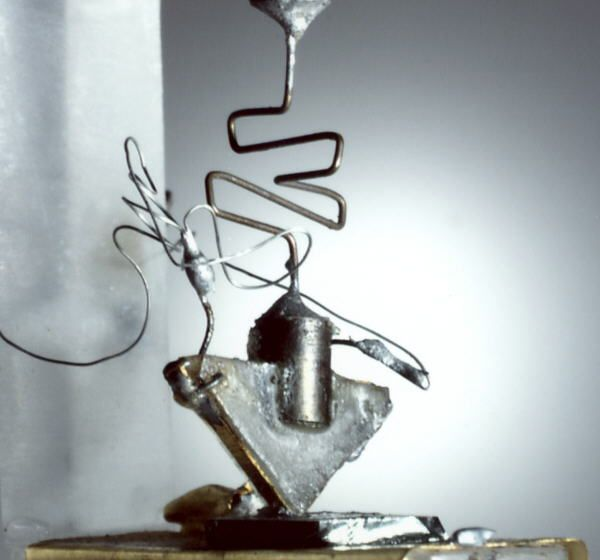
\includegraphics[height=2.63cm]{img/transistor.jpg}\\
    \end{textblock}
\end{frame}

\begin{frame}[fragile,t]{Tercera Generación - Circuitos Integrados}
% ***** Circuito integrado - Robert Noyce 1958
    \begin{textblock}{90}(3,12)
    \begin{itemize}
    \setlength\itemsep{0.2cm}
    \item<1-> IBM 7094 / IBM 1401 (incompatibles)\\
    \small \textcolor{gray}{ \textcolor{naranjauca}{IBM 7094}: Un triturador de números con aritmética binaria y palabras de 36 bits.\\
    \textcolor{naranjauca}{IBM 1401}: Un procesador de entrada/salida con aritmética decimal de longitud variable.\\
    \bigskip
    \textcolor{verdeuca}{\textbf{Dos programas completamente\\ distintos para ambas máquinas.}}}
    \bigskip
    \item<2-> IBM System/360 (1964)\\
    \textbf{Familia de máquinas con el mismo lenguaje ensamblador}\\ 
    \small \textcolor{gray}{
    Podía correr múltiples programas, de a uno por vez.\\
    Arquitectura microprogramada, podía emular a otras máquinas (Las 7094 y 1401).\\
    Gran espacio de direcciones 16MB.}
    \end{itemize}
    \end{textblock}
    \begin{textblock}{100}(100,5)
    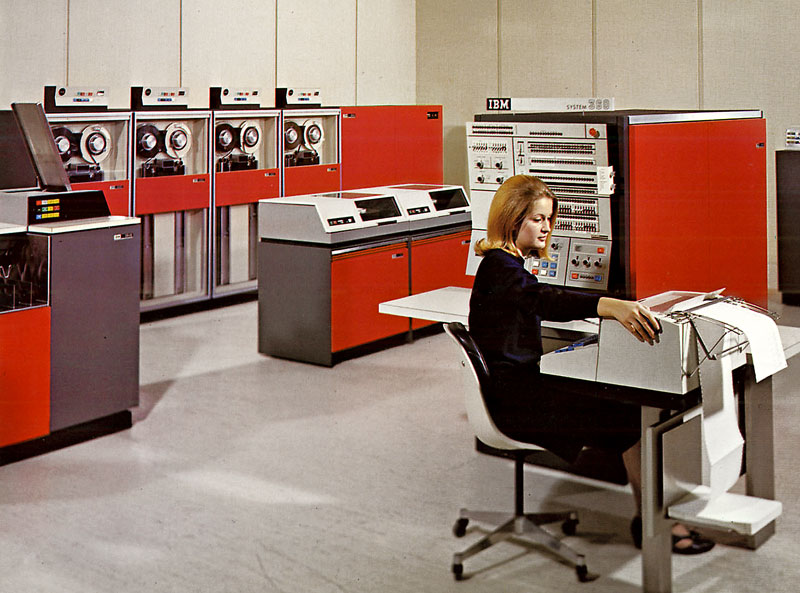
\includegraphics[width=5cm]{img/IBM360.jpg}\\
    \vspace{0.1cm}
    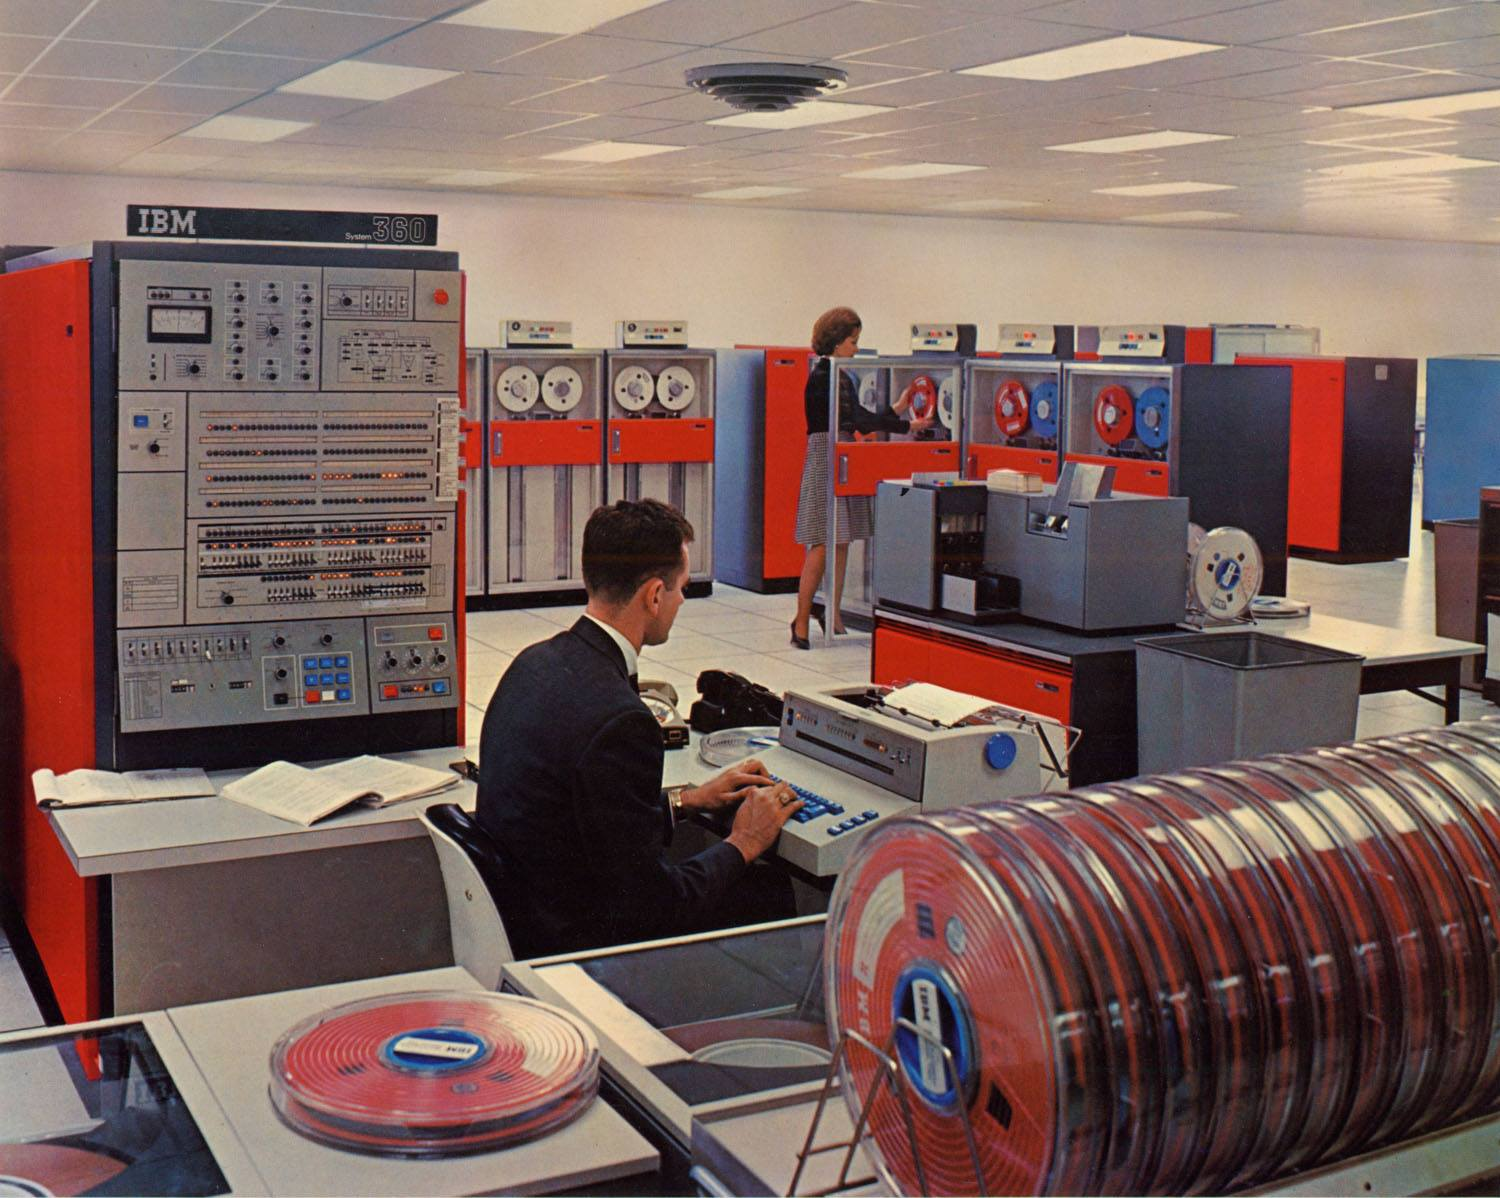
\includegraphics[width=5cm]{img/IBM360x.jpg}\\
    \end{textblock}
\end{frame}

\begin{frame}[fragile,t]{Cuarta Generación - Integración a gran escala}
% ***** VLSI (very large scale integration)
    \begin{textblock}{90}(5,12)
    Reducción de costos: \textcolor{naranjauca}{de departamentos de computación a computadoras personales}.\\
    \textbf{¡Una persona podía tener una computadora!}\\
    \begin{itemize}
    \setlength\itemsep{0.1cm}
    \small
    \item<2-> Las primeras computadoras personales se vendían en kit para armar.
    \item<3-> No contenían software, ya que el usuario lo programaba.
    \item<4-> Aparece el primer sistema operativo CP/M escrito por Gary Kildall para el intel 8080 (1974).
    \item<5-> Aparece Apple y luego Apple II que se populariza entre escuelas y usuarios caseros (1976).
    \item<6-> La IBM PC (1981).\\
    \textcolor{gray}{
    Armada con componentes comerciales.
    Los planos de la máquina eran públicos para que los usuarios hicieran hardware y lo conectasen.
    Con el tiempo aparecen clones más económicos que los de IBM.}
    \end{itemize}
    \end{textblock}
    \begin{textblock}{100}(100,5)
    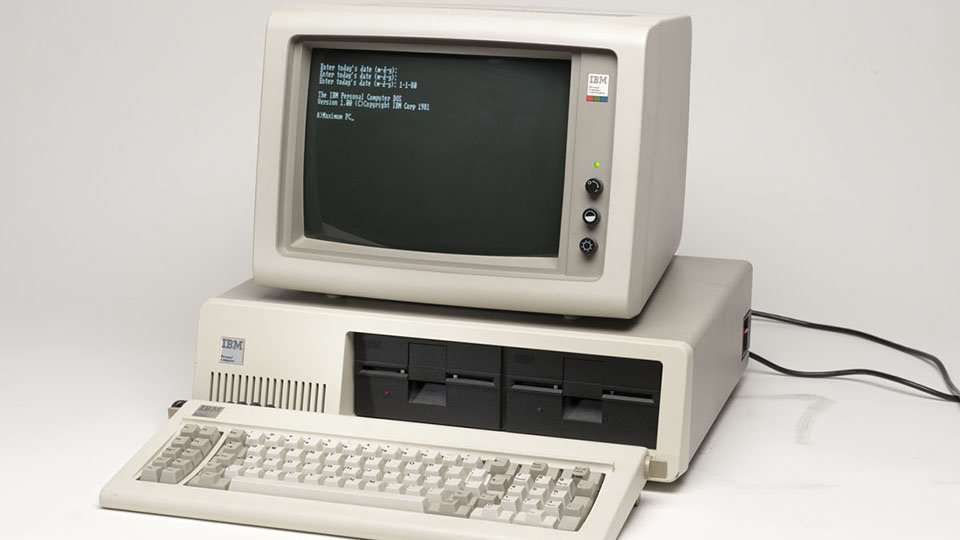
\includegraphics[width=5.2cm]{img/IBMPC.jpg}\\
    \vspace{0.1cm}
    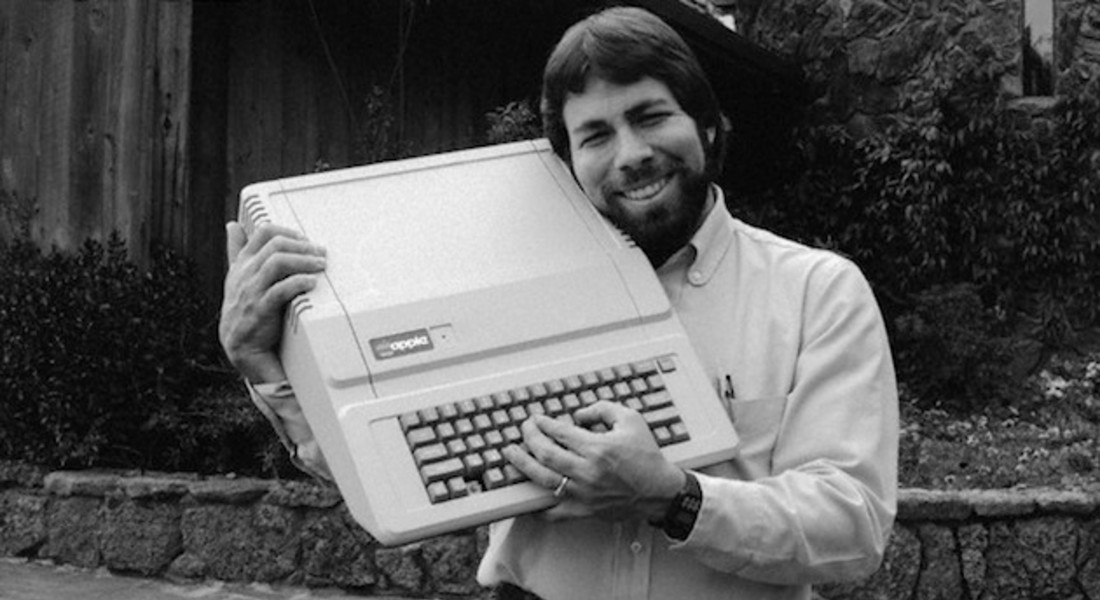
\includegraphics[width=5.2cm]{img/steve-wozniak-apple-1.jpg}\\
    \vspace{0.1cm}
    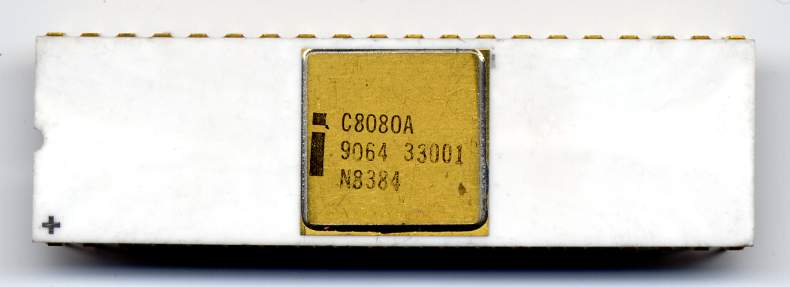
\includegraphics[width=5.2cm]{img/Intel_C8080A.jpg}\\
    \end{textblock}
\end{frame}

\begin{frame}[fragile,t]{ARPANET\\ 1970}
    \begin{textblock}{100}(20,10)
    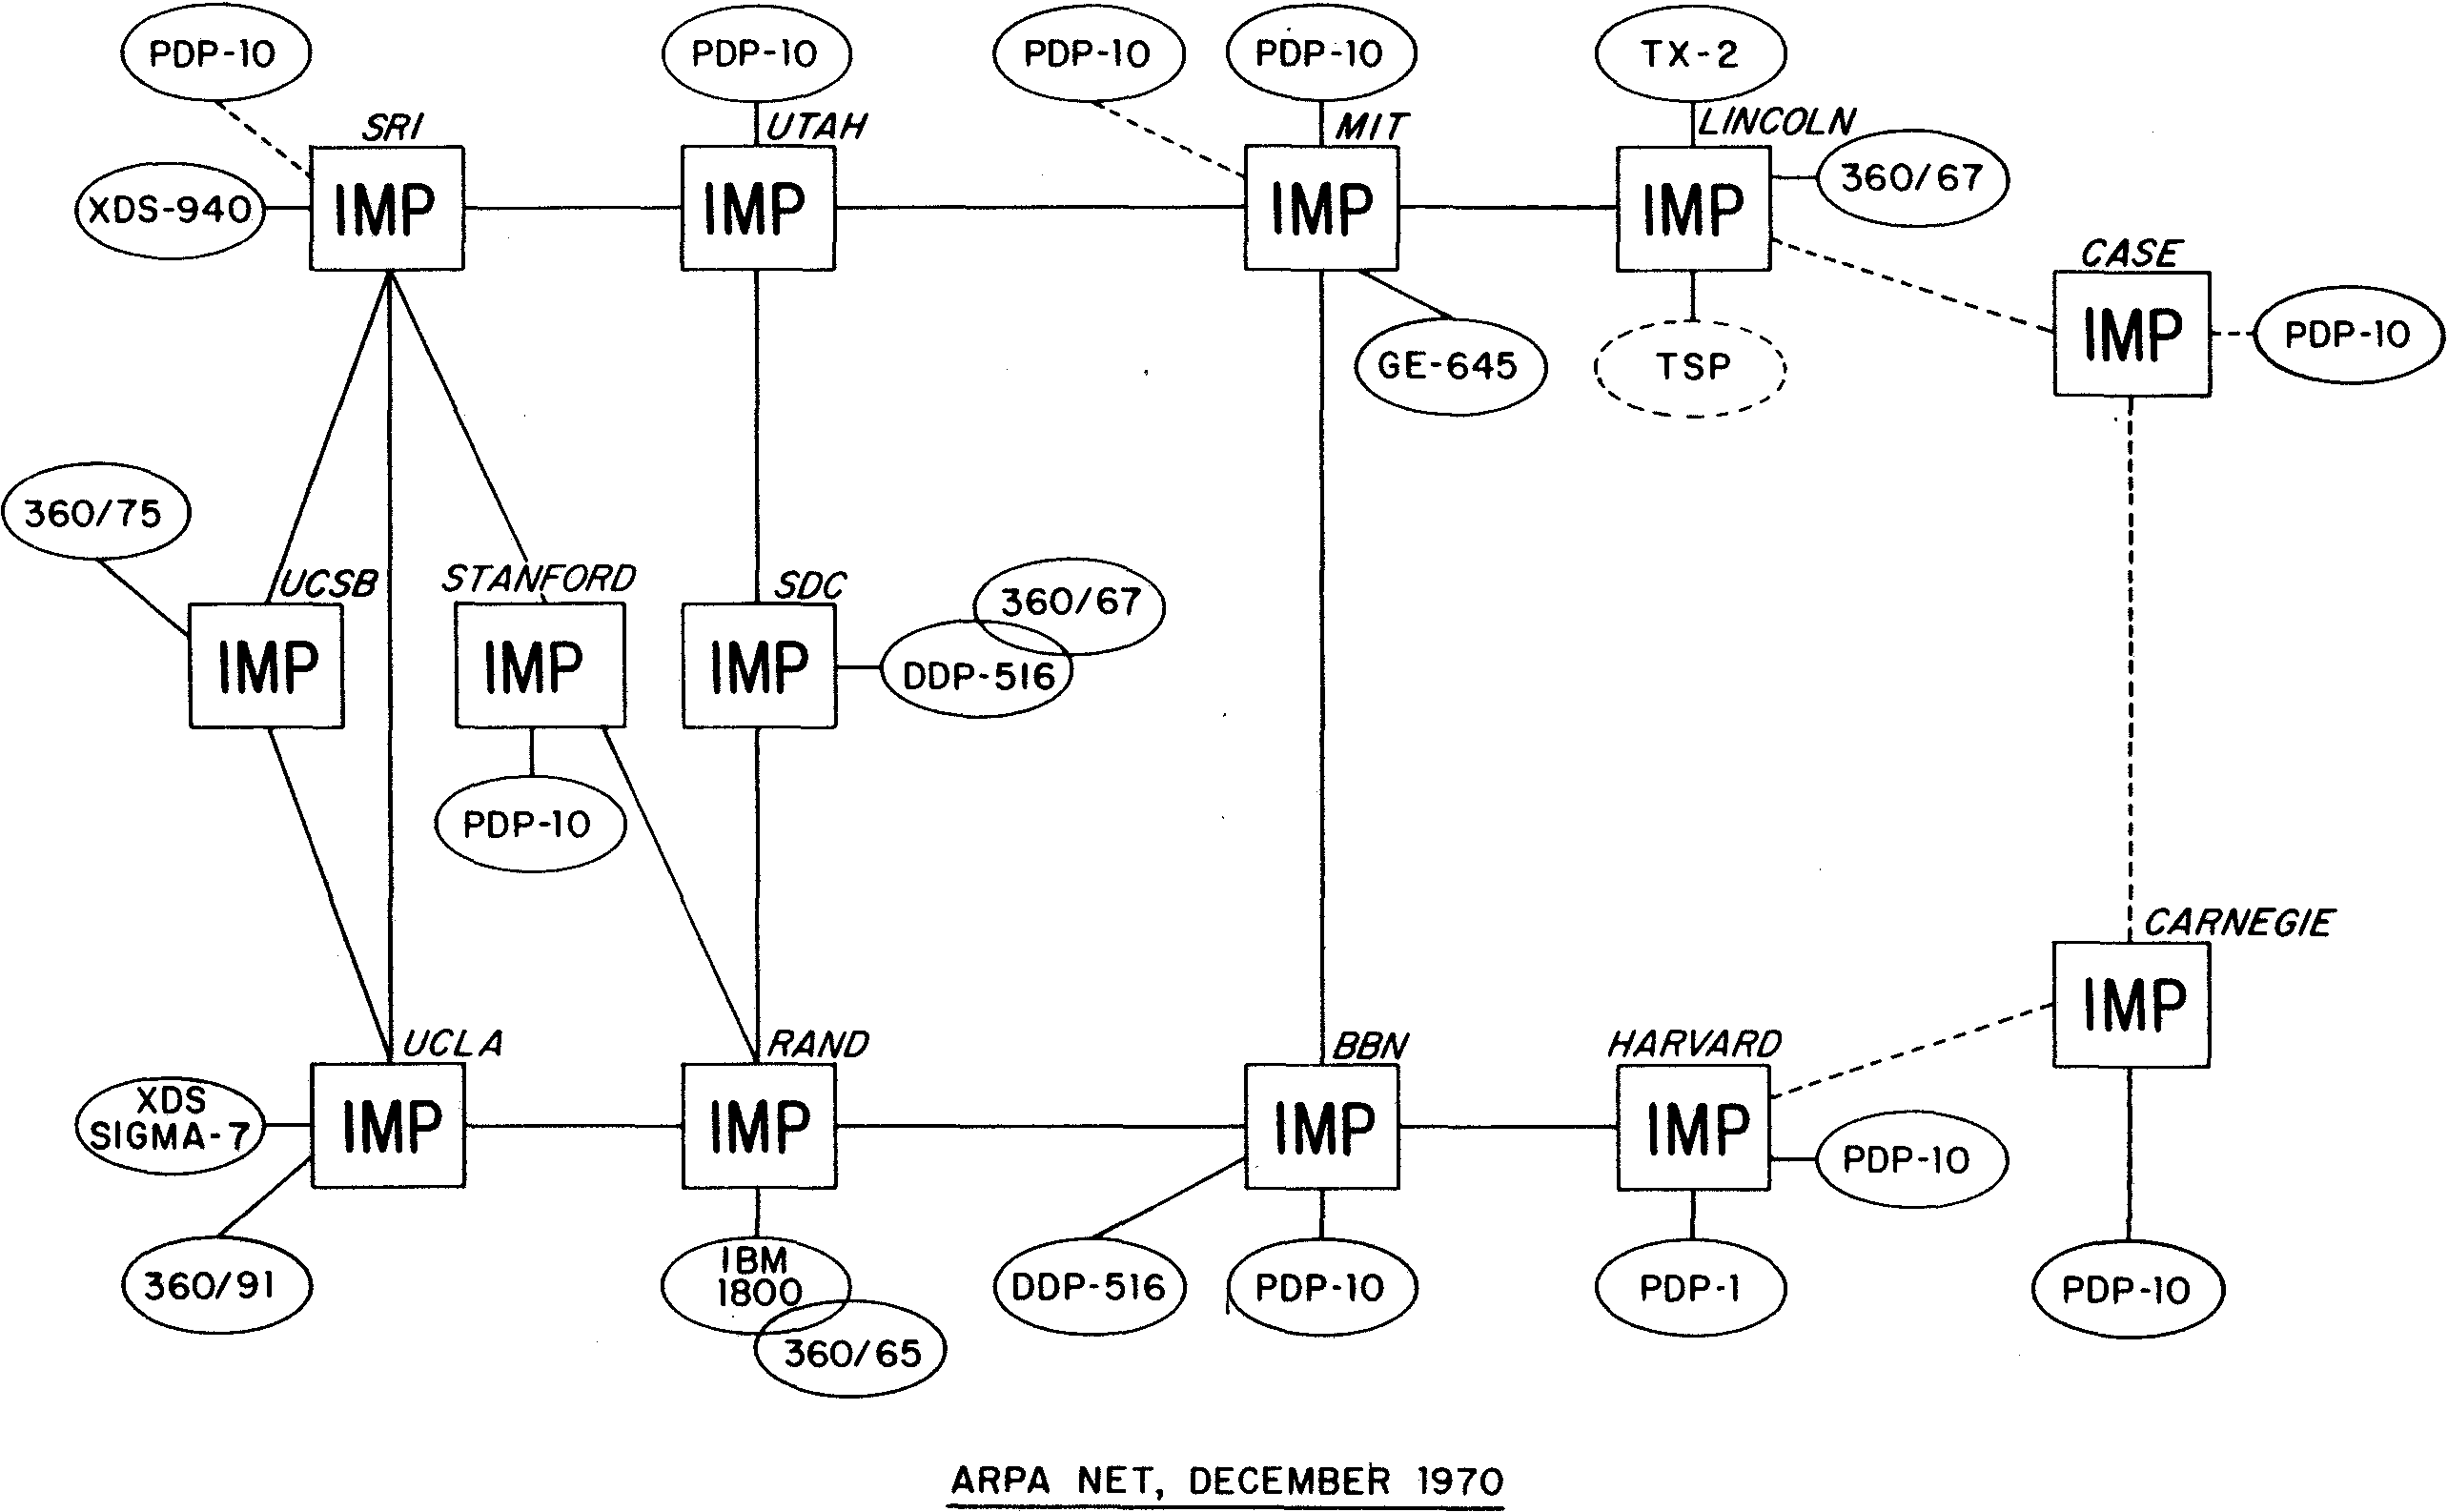
\includegraphics[scale=0.14]{img/arpanet1970.png}\\
    \end{textblock}
    \begin{textblock}{100}(110,87)
    \tiny \textbf{Fuente:} ARPANET Completion Report - January 4, 1978
    \end{textblock}
\end{frame}

\begin{frame}[fragile,t]{ARPANET\\ 1977}
    \begin{textblock}{100}(25,1)
    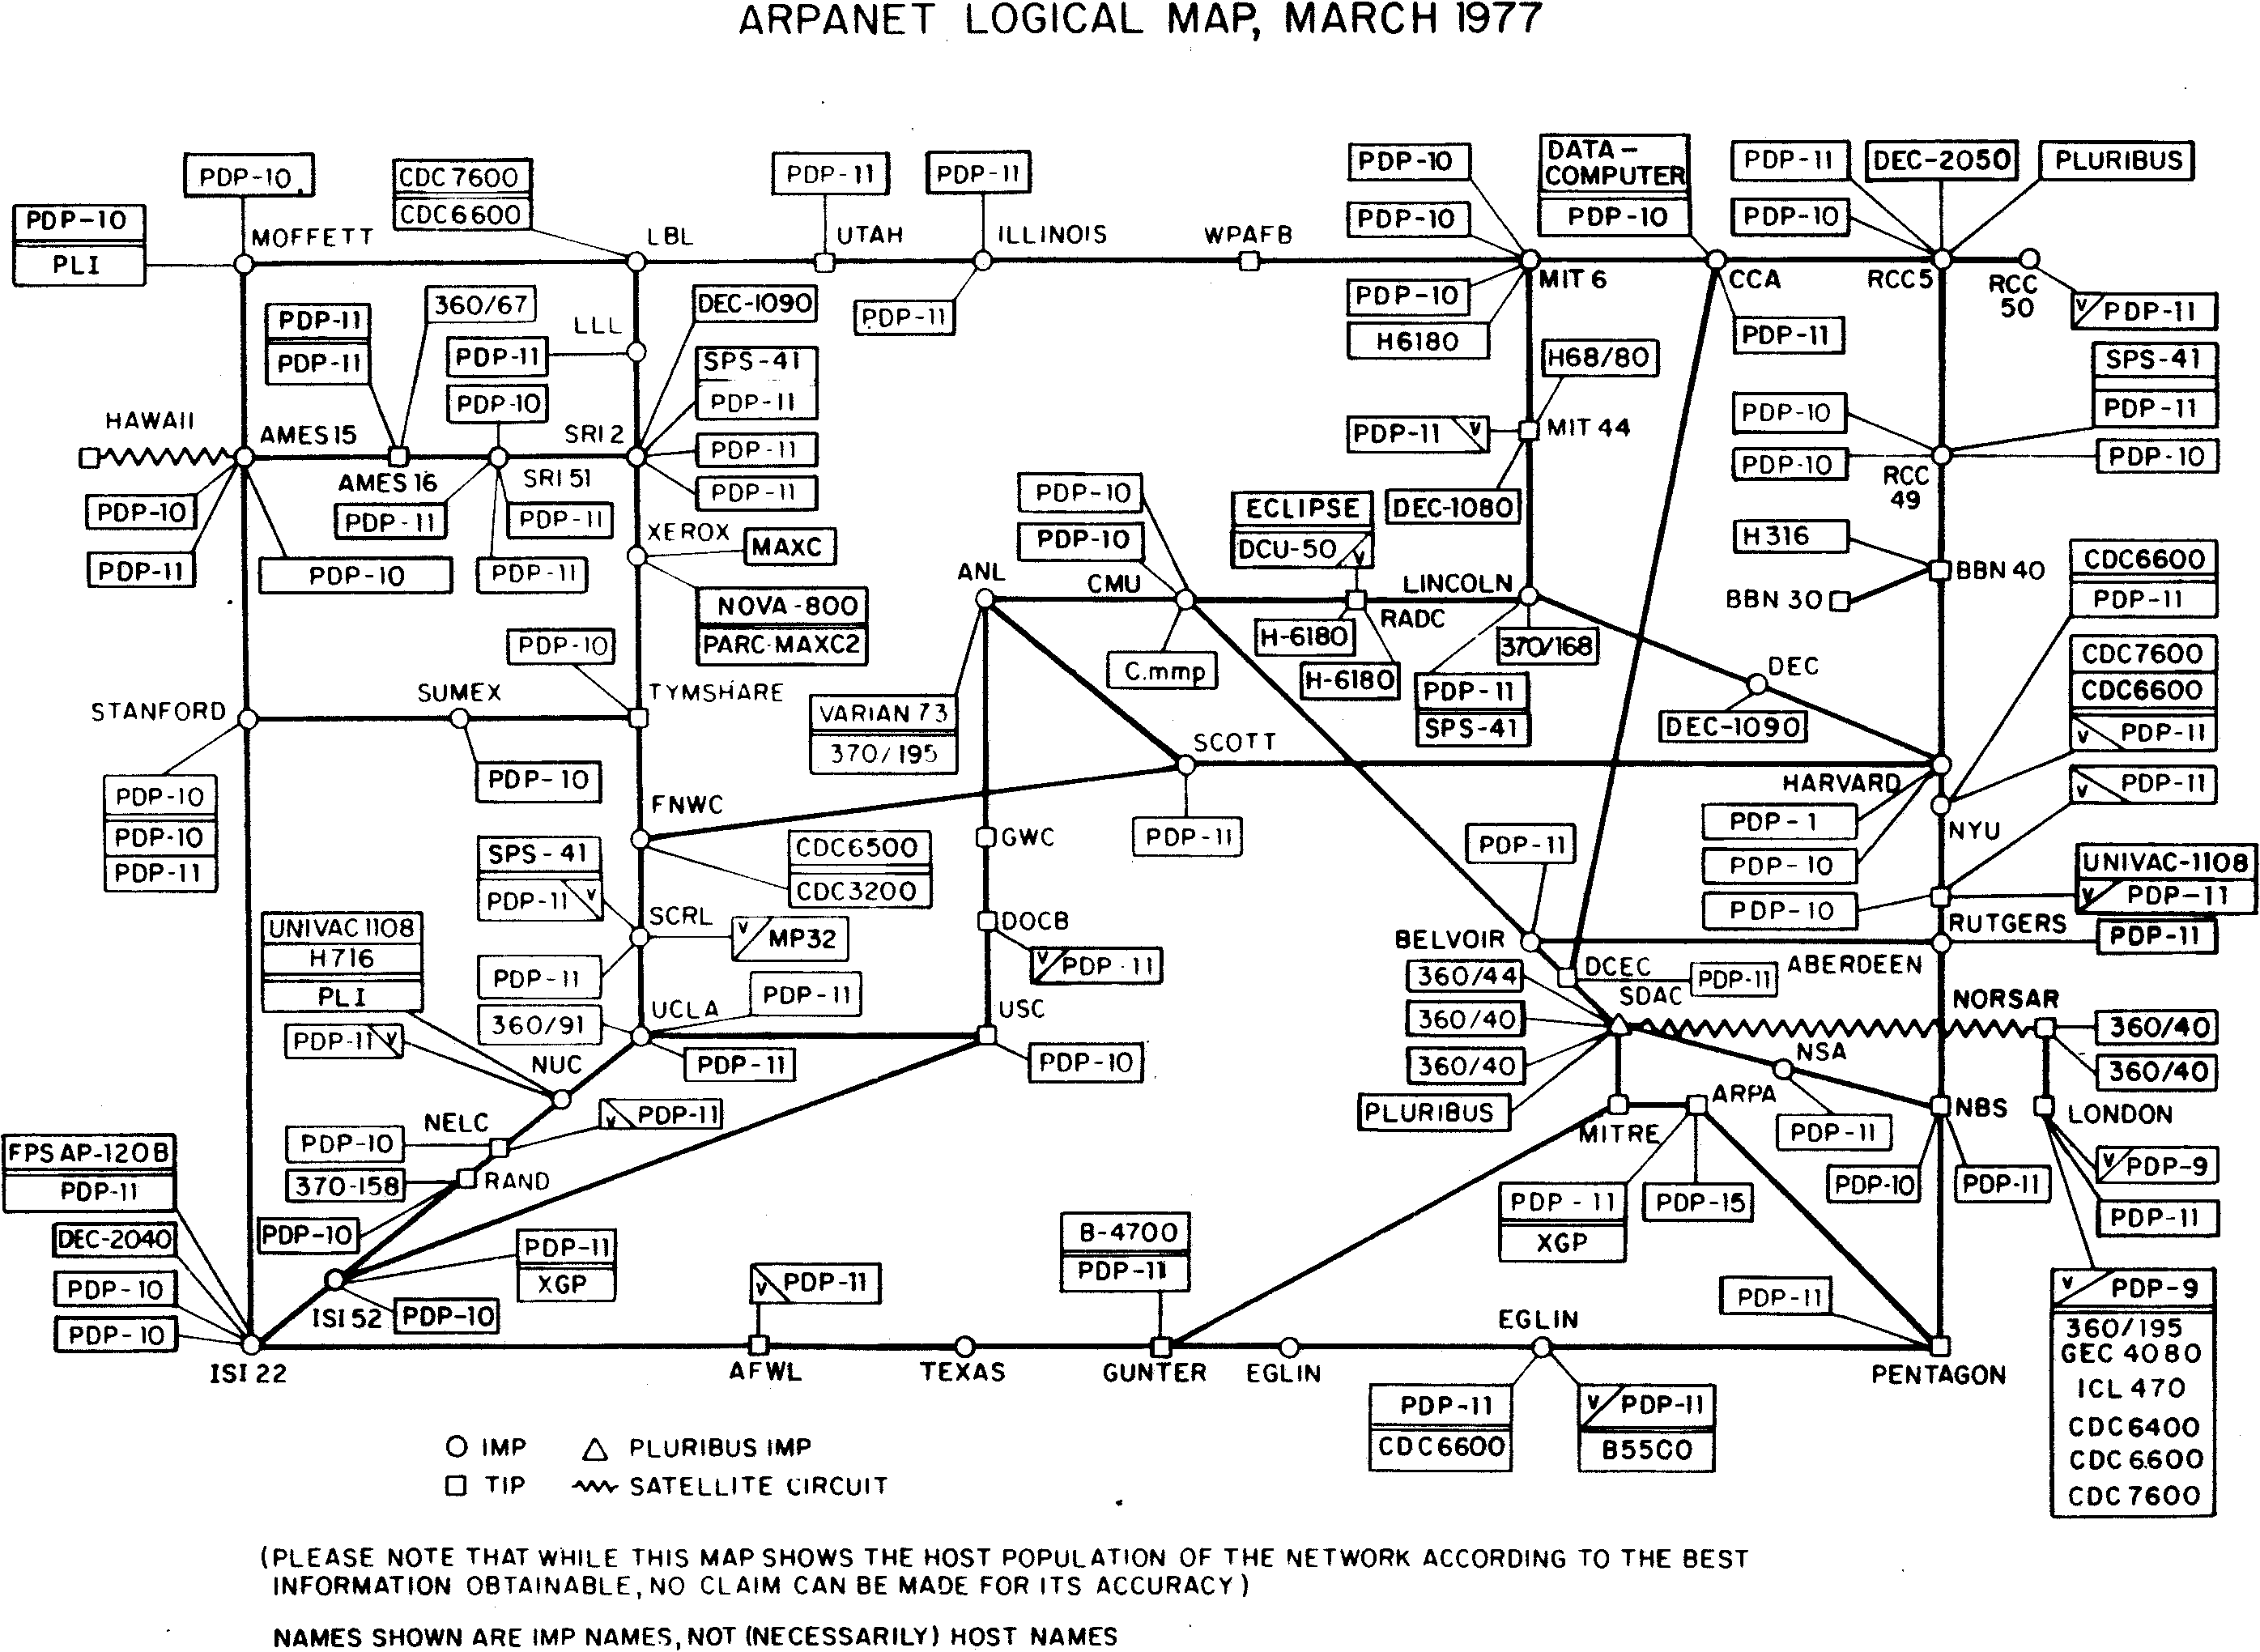
\includegraphics[scale=0.122]{img/arpanet1977.png}\\
    \end{textblock}
    \begin{textblock}{100}(110,87)
    \tiny \textbf{Fuente:} ARPANET Completion Report - January 4, 1978
    \end{textblock}
\end{frame}

\begin{frame}[fragile,t]{Evolución del rendimiento de procesadores: ``Ley'' de Moore}
    \vspace{-0.3cm}
    \begin{center}
    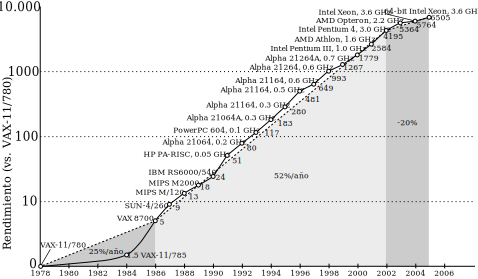
\includegraphics[scale=1]{img/processor-performance_ES.pdf}
    \end{center}
    \vspace{-0.5cm}
    \tiny \textbf{Fuente:} Computer Organization and Design. The Hardware / Software Interface. David A. Patterson, John L. Hennessy. Fourth Edition. Morgan Kaufmann. (pag. 42)
\end{frame}

\begin{frame}[fragile,t]{Relación entre la velocidad de la memoria y el CPU}
    \begin{center}
    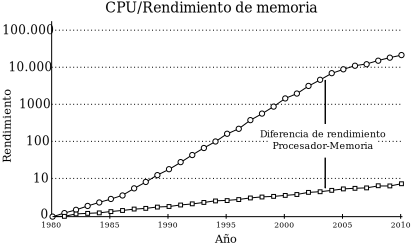
\includegraphics[scale=1]{img/cpu_vs_memory_ES.pdf}
    \end{center}
\end{frame}

\begin{frame}[fragile]
    \frametitle{Bibliografía}
    \begin{itemize}
     \setlength\itemsep{0.5cm}
    \item[-] \small Tanenbaum, “Organización de Computadoras. Un Enfoque Estructurado”, 4ta Edición, 2000.\\
    \begin{itemize}
     \item \textbf{Capitulo 1 - Introducción}\\
     \begin{itemize}
      \item 1.2 - Acontencimientos importantes en arquitectura de computadoras.
      \item 1.3 - El zoológico de las computadoras.
     \end{itemize}
    \end{itemize}
    \item[-] \small Null, “Essentials of Computer Organization and Architecture”, 5th Edition, 2018.\\
    \begin{itemize}
    \item \textbf{Chapter 1 - Introduction}
     \begin{itemize}
        \item 5.1.5 - Historical Development
     \end{itemize}
    \end{itemize}
%     \item[-] \small Silberschatz, “Fundamentos de Sistemas Operativos”, 7ma Edición, 2006.\\
%     \item[-] \small Tanenbaum, “Modern Operating Systems”, 4th Edition, 2015.\\
    \end{itemize}
\end{frame}

\begin{frame}[plain]
    \begin{center}
    \vspace{2cm}
    \huge ¡Gracias!\\
    \vspace{2cm}
    \normalsize Recuerden leer los comentarios adjuntos\\ en cada clase por aclaraciones.
    \end{center}
\end{frame}

\end{document}

% % % % % % % % % % % % % % % % % % 
% EJEMPLOS:

\begin{frame}[fragile]
    \frametitle{Bla}
    \begin{itemize}
    \item[-] Bla bla \textbf{ble} bla bla
    \item[-] Bla bla \textbf{ble} bla bla
    \end{itemize}
\end{frame}

\begin{frame}[fragile]
    \frametitle{Bla}
    \begin{block}{\texttt{BLA}}
    Bla Bla
    \end{block}
    \begin{multicols}{2}
    \begin{tabular}{ll}
    la & la \\
    \end{tabular}
    \columnbreak
    \begin{tabular}{ll}
    la & la \\
    \end{tabular}
    \end{multicols}
\end{frame}

\begin{frame}
    \frametitle{Bla}
    \begin{itemize}
    \item Bla bla
    \begin{center}
    \includegraphics[scale=0.7]{img/struct_aling.pdf}
    \end{center}
    Bla bla
    \end{itemize}
\end{frame}

\begin{frame}[fragile]
    \frametitle{Bla}
    \begin{textblock}{100}(10,10)
    Bla
    \end{textblock}
\end{frame}

\end{document}

